\documentclass[twoside]{book}

% Packages required by doxygen
\usepackage{calc}
\usepackage{doxygen}
\usepackage{graphicx}
\usepackage[utf8]{inputenc}
\usepackage{makeidx}
\usepackage{multicol}
\usepackage{multirow}
\usepackage{textcomp}
\usepackage[table]{xcolor}

% NLS support packages
\usepackage{polski}
\usepackage[T1]{fontenc}

% Font selection
\usepackage[T1]{fontenc}
\usepackage{mathptmx}
\usepackage[scaled=.90]{helvet}
\usepackage{courier}
\usepackage{amssymb}
\usepackage{sectsty}
\renewcommand{\familydefault}{\sfdefault}
\allsectionsfont{%
  \fontseries{bc}\selectfont%
  \color{darkgray}%
}
\renewcommand{\DoxyLabelFont}{%
  \fontseries{bc}\selectfont%
  \color{darkgray}%
}

% Page & text layout
\usepackage{geometry}
\geometry{%
  a4paper,%
  top=2.5cm,%
  bottom=2.5cm,%
  left=2.5cm,%
  right=2.5cm%
}
\tolerance=750
\hfuzz=15pt
\hbadness=750
\setlength{\emergencystretch}{15pt}
\setlength{\parindent}{0cm}
\setlength{\parskip}{0.2cm}
\makeatletter
\renewcommand{\paragraph}{%
  \@startsection{paragraph}{4}{0ex}{-1.0ex}{1.0ex}{%
    \normalfont\normalsize\bfseries\SS@parafont%
  }%
}
\renewcommand{\subparagraph}{%
  \@startsection{subparagraph}{5}{0ex}{-1.0ex}{1.0ex}{%
    \normalfont\normalsize\bfseries\SS@subparafont%
  }%
}
\makeatother

% Headers & footers
\usepackage{fancyhdr}
\pagestyle{fancyplain}
\fancyhead[LE]{\fancyplain{}{\bfseries\thepage}}
\fancyhead[CE]{\fancyplain{}{}}
\fancyhead[RE]{\fancyplain{}{\bfseries\leftmark}}
\fancyhead[LO]{\fancyplain{}{\bfseries\rightmark}}
\fancyhead[CO]{\fancyplain{}{}}
\fancyhead[RO]{\fancyplain{}{\bfseries\thepage}}
\fancyfoot[LE]{\fancyplain{}{}}
\fancyfoot[CE]{\fancyplain{}{}}
\fancyfoot[RE]{\fancyplain{}{\bfseries\scriptsize Wygenerowano N, 15 maj 2016 17\-:48\-:18 dla Średniowiecze programem Doxygen }}
\fancyfoot[LO]{\fancyplain{}{\bfseries\scriptsize Wygenerowano N, 15 maj 2016 17\-:48\-:18 dla Średniowiecze programem Doxygen }}
\fancyfoot[CO]{\fancyplain{}{}}
\fancyfoot[RO]{\fancyplain{}{}}
\renewcommand{\footrulewidth}{0.4pt}
\renewcommand{\chaptermark}[1]{%
  \markboth{#1}{}%
}
\renewcommand{\sectionmark}[1]{%
  \markright{\thesection\ #1}%
}

% Indices & bibliography
\usepackage{natbib}
\usepackage[titles]{tocloft}
\setcounter{tocdepth}{3}
\setcounter{secnumdepth}{5}
\makeindex

% Hyperlinks (required, but should be loaded last)
\usepackage{ifpdf}
\ifpdf
  \usepackage[pdftex,pagebackref=true]{hyperref}
\else
  \usepackage[ps2pdf,pagebackref=true]{hyperref}
\fi
\hypersetup{%
  colorlinks=true,%
  linkcolor=blue,%
  citecolor=blue,%
  unicode%
}

% Custom commands
\newcommand{\clearemptydoublepage}{%
  \newpage{\pagestyle{empty}\cleardoublepage}%
}


%===== C O N T E N T S =====

\begin{document}

% Titlepage & ToC
\hypersetup{pageanchor=false}
\pagenumbering{roman}
\begin{titlepage}
\vspace*{7cm}
\begin{center}%
{\Large Średniowiecze }\\
\vspace*{1cm}
{\large Wygenerowano przez Doxygen 1.8.6}\\
\vspace*{0.5cm}
{\small N, 15 maj 2016 17:48:18}\\
\end{center}
\end{titlepage}
\clearemptydoublepage
\tableofcontents
\clearemptydoublepage
\pagenumbering{arabic}
\hypersetup{pageanchor=true}

%--- Begin generated contents ---
\chapter{Dokumentacja Zadania Średniowiecze}
\label{index}\hypertarget{index}{}\section*{Średniowiecze}

Uwaga\-: aktualna treść zadania znajduje się w \href{https://moodle.mimuw.edu.pl/mod/assignment/view.php?id=18178}{\tt Moodle'u}.

\subsubsection*{Opis projektu}

Dużym, trzyczęściowym projektem zaliczeniowym w tym roku jest implementacja deterministycznej turowej gry strategicznej z pełną wiedzą wraz ze sztuczną inteligencją (A\-I). Pierwsza część polega na zaimplementowaniu i przetestowaniu struktur danych oraz protokołu wejścia w programie A\-I. W drugiej części należy stworzyć nic nie robiącą A\-I oraz skrypt bash łączący program interfejsu graficznego i programy A\-I w symulator rozgrywki A\-I vs A\-I, A\-I vs człowiek lub człowiek vs człowiek. W trzeciej i ostatniej części należy stworzyć A\-I potrafiące wygrać przeciwko prostym strategiom.

\subsubsection*{Opis gry}

Gra rozgrywa się na kwadratowej planszy {\ttfamily n$\ast$n} ({\ttfamily 8 $<$ n $<$ 2$^\wedge$31}) i jest przeznaczona dla dwóch graczy wykonujących na zmianę swoje tury (rozpoczynając od pierwszego gracza). Każdy z graczy kontroluje swoje jednostki należące do jednego z trzech typów\-: król, rycerz, chłop. Na początku gry każdy gracz ma 1 króla, 1 chłopa i 2 rycerzy, ustawionych jeden obok drugiego w poziomej linii na planszy w kolejności król, chłop, rycerz, rycerz. Początkowe ustawienie jednostek następuje poprzez wylosowanie pozycji królów spośród pierwszych {\ttfamily n-\/3} kolumn, tak aby królowie byli od siebie oddaleni o co najmniej 8 w metryce maksimum.

Podczas każdej tury gracz może ruszyć raz każdą swoją jednostką. Ruch składa się z przesunięcia jej o 1 pole pionowo, poziomo, na skos lub wykonania akcji (tylko przez chłopa). Gdy jednostka ruszy się na pole zajmowane przez inną jednostkę, następuje walka. Gdy walczą ze sobą dwie jednostki tego samego typu, obie giną. W przeciwnym wypadku rycerz pokonuje króla lub chłopa, a król pokonuje chłopa. Nie można ruszyć swojej jednostki na pole zajmowane przez inną swoją jednostkę (aczkolwiek można najpierw przesunąć jedną jednostkę, a drugą później przesunąć na zwolnione miejsce w tej samej turze). Akcją możliwą do wykonania przez chłopa jest wyprodukowanie nowego rycerza albo chłopa na jednym z sąsiednich (pionowo, poziomo lub po skosie) wolnych pól, pod warunkiem że chłop stał w miejscu, nie wykonując akcji przez poprzednie 2 tury. Innymi słowy chłop, który ruszył się w turze {\ttfamily k}, a potem się już nie ruszał, może dopiero wyprodukować jednostkę w turze {\ttfamily k+3}, następnie {\ttfamily k+6} itd. Nowymi jednostkami można się ruszać od razu po wyprodukowaniu (tj. gdy zostały wyprodukowane w turze {\ttfamily k}, to traktowane są jakby ostatnio wykonały ruch w turze {\ttfamily k-\/1}). Chłop, który od początku gry (tura 1) się nie ruszał, może wyprodukować pierwszą jednostkę w turze 3, a każda jednostka na początku gry może się od razu ruszyć.

Gra kończy się w momencie, gdy król jednego z graczy zginie lub po {\ttfamily k}-\/tej ({\ttfamily 1 $<$= k $<$ 2$^\wedge$31}) turze drugiego gracza. Wygrywa gracz mający jedynego żywego króla. W przeciwnym wypadku mamy remis.

\subsection*{Część 1}

Napisz program interpretujący protokół komunikacyjny gracza i obsługujący wiadomości dostawane na standardowym wejściu od obu graczy (w tym obie wiadomości {\ttfamily I\-N\-I\-T}, o czym za chwilę). Po każdym ruchu (dokładniej, po każdej wiadomości innej niż {\ttfamily E\-N\-D\-\_\-\-T\-U\-R\-N}) program powinien wypisać na standardowe wyjście tekstową reprezentację górnego lewego rogu planszy (górne {\ttfamily 10$\ast$10} pól, chyba że plansza jest mniejsza). Jednostki pierwszego gracza powinny być zaznaczone wielkimi literami {\ttfamily K}, {\ttfamily R}, {\ttfamily C} (odpowiednio król, rycerz, chłop), jednostki drugiego gracza małymi literami {\ttfamily k}, {\ttfamily r}, {\ttfamily c}, a puste pola kropką. Przykład planszy\-: \begin{DoxyVerb}..........
.KRRC.....
..........
..........
....r.r...
.....k....
.....c....
..........
..........
..........
\end{DoxyVerb}


Na wyjściu nie powinno być żadnych dodatkowych znaków. Po każdej planszy powinna zostać wypisana pojedyncza pusta linia.

\subsubsection*{Protokół komunikacyjny gracza}

Program powinien obsługiwać następujące polecenia\-: {\ttfamily I\-N\-I\-T n k p x1 y1 x2 y2} – informacja o stanie początkowym gry, osobno dla każdego gracza\-: n – wielkość planszy, k – maksymalna liczba tur (na gracza), p – numer gracza (1 lub 2), (x1, y1) – początkowe współrzędne króla pierwszego gracza, (x2, y2) – początkowe współrzędne króla drugiego gracza; {\ttfamily M\-O\-V\-E x1 y1 x2 y2} – ruch jednostką z pozycji (x1, y1) na (x2, y2); {\ttfamily P\-R\-O\-D\-U\-C\-E\-\_\-\-K\-N\-I\-G\-H\-T x1 y1 x2 y2} – wyprodukowanie przez chłopa znajdującego się na polu (x1, y1) rycerza na sąsiednie pole (x2, y2); {\ttfamily P\-R\-O\-D\-U\-C\-E\-\_\-\-P\-E\-A\-S\-A\-N\-T x1 y1 x2 y2} – wyprodukowanie przez chłopa znajdującego się na polu (x1, y1) chłopa na sąsiednie pole (x2, y2); {\ttfamily E\-N\-D\-\_\-\-T\-U\-R\-N} – informacja o końcu tury obecnie poruszającego się gracza.

Każda wiadomość musi być zakończona znakiem nowej linii ({\ttfamily \textbackslash{}n}), a poszczególne jej argumenty mogą być oddzielone wyłącznie pojedynczymi spacjami. Na końcu wiadomości nie ma spacji.

Górny lewy róg planszy ma współrzędne (1, 1). Współrzędna {\ttfamily x} to numer kolumny, a współrzędna {\ttfamily y} to numer wiersza.

\subsubsection*{Wyjście programu}

Program powinien wykrywać, kiedy gra się zakończyła i wtedy po przeprowadzeniu ostatniego ruchu wypisać na standardowe wyjście diagnostyczne ({\ttfamily stderr}) jeden z komunikatów\-: {\ttfamily player 1 won}, {\ttfamily player 2 won} lub {\ttfamily draw} i zakończyć się z kodem 0.

W przypadku otrzymania niepoprawnego wejścia program powinien wypisać na standardowe wyjście diagnostyczne {\ttfamily input error} i zakończyć się z kodem błędu 42. Żadne poprawne polecenie nie jest dłuższe niż 100 znaków, ale program powinien się poprawnie zakończyć nawet w przypadku dowolnie długiej linii (uwaga na {\ttfamily gets} albo {\ttfamily scanf(\char`\"{}\%s\char`\"{})}).

\subsubsection*{Implementacja}

W repozytorium X\-X\-X znajduje się wstępna implementacja rozwiązania tego zadania. Zadanie to należy oddawać właśnie przez to repozytorium. W repozytorium, które pobierzesz, będą znajdowały się następujące pliki\-: {\itshape \hyperlink{middle__ages_8c}{src/middle\-\_\-ages.\-c}} – główny plik programu, w którym wczytujemy dane wejściowe i uruchamiamy silnik gry; plik ten nie powinien znać szczegółów implementacji silnika gry; {\itshape src/engine.\-c} – plik biblioteki „silnika” gry zawierający wszystkie struktury i funkcje potrzebne do przeprowadzenia rozgrywki; {\itshape \hyperlink{engine_8h}{src/engine.\-h}} – plik nagłówkowy biblioteki silnika gry; {\itshape src/parse.\-c} – plik biblioteki wczytującej i parsującej polecenia; {\itshape \hyperlink{parse_8h}{src/parse.\-h}} – plik nagłówkowy biblioteki wczytującej i parsującej polecenia; {\itshape C\-Make\-Lists.\-txt} – plik konfiguracyjny C\-Make'a; {\itshape Doxyfile.\-in} – plik konfiguracyjny Doxygena; {\itshape Main\-Page.\-dox} – strona główna dokumentacji Doxygena.

Projekt można zaimportować do C\-Liona i tam zbudować. Można też zbudować go (będąc w katalogu głównym) przy użyciu poleceń\-: \begin{DoxyVerb}mkdir build
cd build
cmake ..
\end{DoxyVerb}


Po wywołaniu {\ttfamily make} w katalogu {\itshape build} pojawi się wykonywalny plik {\itshape middle\-\_\-ages}. Twoim zadaniem jest rozbudowanie tego projektu tak, aby program {\itshape middle\-\_\-ages} reagował na polecenia ze standardowego wejścia zgodnie ze specyfikacją opisaną w sekcji Protokół komunikacyjny gracza$\ast$$\ast$. Projekt może zawierać inne pliki niż wyżej wymienione, a zaproponowane funkcjonalności poszczególnych plików można dalej dzielić na moduły (ale nie łączyć).

\subsubsection*{Dokumentacja Doxygen}

Polecenie {\ttfamily make doc} wywołane w katalogu {\itshape build} generuje dokumentację Doxygena całego projektu na podstawie komentarzy umieszczonych w poszczególnych plikach. Twoje rozwiązanie powinno zawierać komentarze Doxygena co najmniej do każdego pliku oraz do wszystkich funkcji eksportowanych na zewnątrz pliku, w którym się znajdują.

\subsubsection*{Punktacja}

Za w pełni poprawnie rozwiązane zadanie można uzyskać 20 pkt. Za złe działanie programu na planszach większych niż 1000 x 1000 można stracić co najwyżej 8 pkt. Za złe parsowanie niepoprawnych poleceń można stracić co najwyżej 3 pkt. Za wycieki pamięci można stracić co najwyżej 6 pkt. Za błędy związane z dokumentacją Doxygen można stracić co najwyżej 3 pkt. Za zły styl kodowania można stracić co najwyżej 3 pkt. 
\chapter{Indeks struktur danych}
\section{Struktury danych}
Tutaj znajdują się struktury danych wraz z ich krótkimi opisami\-:\begin{DoxyCompactList}
\item\contentsline{section}{\hyperlink{structdef__command}{def\-\_\-command} }{\pageref{structdef__command}}{}
\item\contentsline{section}{\hyperlink{structinput__parameters}{input\-\_\-parameters} \\*This structure include input parameters }{\pageref{structinput__parameters}}{}
\item\contentsline{section}{\hyperlink{structline}{line} \\*Structure of single line }{\pageref{structline}}{}
\item\contentsline{section}{\hyperlink{structlist__of__lines}{list\-\_\-of\-\_\-lines} \\*Structure of \hyperlink{structlist__of__lines}{list\-\_\-of\-\_\-lines} }{\pageref{structlist__of__lines}}{}
\end{DoxyCompactList}

\chapter{Indeks plików}
\section{Lista plików}
Tutaj znajduje się lista wszystkich udokumentowanych plików z ich krótkimi opisami\-:\begin{DoxyCompactList}
\item\contentsline{section}{\hyperlink{engine_8h}{engine.\-h} \\*Interface of game engine }{\pageref{engine_8h}}{}
\item\contentsline{section}{\hyperlink{middle__ages_8c}{middle\-\_\-ages.\-c} \\*Interface of middle\-\_\-ages }{\pageref{middle__ages_8c}}{}
\item\contentsline{section}{\hyperlink{parse_8h}{parse.\-h} \\*Interface of parser }{\pageref{parse_8h}}{}
\end{DoxyCompactList}

\chapter{Dokumentacja struktur danych}
\hypertarget{structdef__command}{\section{Dokumentacja struktury def\-\_\-command}
\label{structdef__command}\index{def\-\_\-command@{def\-\_\-command}}
}
\subsection*{Pola danych}
\begin{DoxyCompactItemize}
\item 
\hypertarget{structdef__command_af8fb01ba8e40c37b8a2e94e77fcc52fb}{char {\bfseries name} \mbox{[}16\mbox{]}}\label{structdef__command_af8fb01ba8e40c37b8a2e94e77fcc52fb}

\item 
\hypertarget{structdef__command_a8894767984f2875f9cbcde28a9d2658a}{int {\bfseries data} \mbox{[}7\mbox{]}}\label{structdef__command_a8894767984f2875f9cbcde28a9d2658a}

\item 
\hypertarget{structdef__command_a0ce0204aa4be8cdd8d04b8bbffbe9b31}{bool {\bfseries correct}}\label{structdef__command_a0ce0204aa4be8cdd8d04b8bbffbe9b31}

\end{DoxyCompactItemize}


Dokumentacja dla tej struktury została wygenerowana z plików\-:\begin{DoxyCompactItemize}
\item 
parse.\-c\item 
\hyperlink{parse_8h}{parse.\-h}\end{DoxyCompactItemize}

\hypertarget{structinput__parameters}{\section{Dokumentacja struktury input\-\_\-parameters}
\label{structinput__parameters}\index{input\-\_\-parameters@{input\-\_\-parameters}}
}


This structure include input parameters.  




{\ttfamily \#include $<$engine.\-h$>$}

\subsection*{Pola danych}
\begin{DoxyCompactItemize}
\item 
\hypertarget{structinput__parameters_ab3a0882ef67c5fb19683671720fcc7a6}{int \hyperlink{structinput__parameters_ab3a0882ef67c5fb19683671720fcc7a6}{n}}\label{structinput__parameters_ab3a0882ef67c5fb19683671720fcc7a6}

\begin{DoxyCompactList}\small\item\em size of map \end{DoxyCompactList}\item 
\hypertarget{structinput__parameters_abb9b1fbe51332fcecfb5a5cd205f047f}{int \hyperlink{structinput__parameters_abb9b1fbe51332fcecfb5a5cd205f047f}{k}}\label{structinput__parameters_abb9b1fbe51332fcecfb5a5cd205f047f}

\begin{DoxyCompactList}\small\item\em maximum amount of turns for every player \end{DoxyCompactList}\item 
\hypertarget{structinput__parameters_a19e44a03729441c732e953a3ca01bc3f}{int \hyperlink{structinput__parameters_a19e44a03729441c732e953a3ca01bc3f}{p1}}\label{structinput__parameters_a19e44a03729441c732e953a3ca01bc3f}

\begin{DoxyCompactList}\small\item\em number of player1 \end{DoxyCompactList}\item 
\hypertarget{structinput__parameters_a5846cf94e253e32101934a964a7c74e1}{int \hyperlink{structinput__parameters_a5846cf94e253e32101934a964a7c74e1}{x1}}\label{structinput__parameters_a5846cf94e253e32101934a964a7c74e1}

\begin{DoxyCompactList}\small\item\em x-\/coordinate of king of player1 \end{DoxyCompactList}\item 
\hypertarget{structinput__parameters_a70e75e8878950f26b029c8bcd867dfb3}{int \hyperlink{structinput__parameters_a70e75e8878950f26b029c8bcd867dfb3}{y1}}\label{structinput__parameters_a70e75e8878950f26b029c8bcd867dfb3}

\begin{DoxyCompactList}\small\item\em y-\/coordinate of king of player1 \end{DoxyCompactList}\item 
\hypertarget{structinput__parameters_aeea7bd44e263a5f8d06384efd3bb5d0e}{int \hyperlink{structinput__parameters_aeea7bd44e263a5f8d06384efd3bb5d0e}{x2}}\label{structinput__parameters_aeea7bd44e263a5f8d06384efd3bb5d0e}

\begin{DoxyCompactList}\small\item\em x-\/coordinates of king of player2 \end{DoxyCompactList}\item 
\hypertarget{structinput__parameters_ae324caf4e1ac82a6baaef8a5234081c3}{int \hyperlink{structinput__parameters_ae324caf4e1ac82a6baaef8a5234081c3}{y2}}\label{structinput__parameters_ae324caf4e1ac82a6baaef8a5234081c3}

\begin{DoxyCompactList}\small\item\em y-\/coordinate of king of player2 \end{DoxyCompactList}\item 
\hypertarget{structinput__parameters_acb0783d0bc4681f5aab137eec42eed08}{int \hyperlink{structinput__parameters_acb0783d0bc4681f5aab137eec42eed08}{p2}}\label{structinput__parameters_acb0783d0bc4681f5aab137eec42eed08}

\begin{DoxyCompactList}\small\item\em number of player2 \end{DoxyCompactList}\end{DoxyCompactItemize}


\subsection{Opis szczegółowy}
This structure include input parameters. 

Dokumentacja dla tej struktury została wygenerowana z plików\-:\begin{DoxyCompactItemize}
\item 
engine.\-c\item 
\hyperlink{engine_8h}{engine.\-h}\end{DoxyCompactItemize}

\hypertarget{structline}{\section{Dokumentacja struktury line}
\label{structline}\index{line@{line}}
}


Structure of single line.  




{\ttfamily \#include $<$engine.\-h$>$}



Diagram współpracy dla line\-:\nopagebreak
\begin{figure}[H]
\begin{center}
\leavevmode
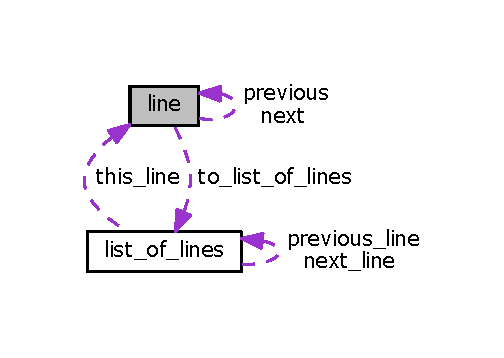
\includegraphics[width=242pt]{structline__coll__graph}
\end{center}
\end{figure}
\subsection*{Pola danych}
\begin{DoxyCompactItemize}
\item 
\hypertarget{structline_a78bdea175fde5dcd9b56fcf091663b42}{bool \hyperlink{structline_a78bdea175fde5dcd9b56fcf091663b42}{king}}\label{structline_a78bdea175fde5dcd9b56fcf091663b42}

\begin{DoxyCompactList}\small\item\em Information about race of unit. \end{DoxyCompactList}\item 
\hypertarget{structline_aa71a3f832987387529bf56948e0c1fbe}{bool \hyperlink{structline_aa71a3f832987387529bf56948e0c1fbe}{knight}}\label{structline_aa71a3f832987387529bf56948e0c1fbe}

\begin{DoxyCompactList}\small\item\em Information about race of unit. \end{DoxyCompactList}\item 
\hypertarget{structline_a89b63cb266efa1ebcb62489dfecc04e9}{bool \hyperlink{structline_a89b63cb266efa1ebcb62489dfecc04e9}{peasant}}\label{structline_a89b63cb266efa1ebcb62489dfecc04e9}

\begin{DoxyCompactList}\small\item\em Information about race of unit. \end{DoxyCompactList}\item 
\hypertarget{structline_ac4e499f0d40aaafc5771fe608f715391}{int {\bfseries pos\-\_\-x}}\label{structline_ac4e499f0d40aaafc5771fe608f715391}

\item 
\hypertarget{structline_a0a348a46dffa63ec70910c92617ed28f}{int {\bfseries player\-\_\-number}}\label{structline_a0a348a46dffa63ec70910c92617ed28f}

\item 
\hypertarget{structline_aa78f4ee2c8381d55e1ba9cbe9ae9554d}{int {\bfseries last\-\_\-move\-\_\-or\-\_\-action}}\label{structline_aa78f4ee2c8381d55e1ba9cbe9ae9554d}

\item 
\hypertarget{structline_a018f1985c87241c864aef6e5da9aa952}{struct \hyperlink{structline}{line} $\ast$ \hyperlink{structline_a018f1985c87241c864aef6e5da9aa952}{next}}\label{structline_a018f1985c87241c864aef6e5da9aa952}

\begin{DoxyCompactList}\small\item\em Indicator to next unit in line. \end{DoxyCompactList}\item 
\hypertarget{structline_abb721ad888ffdb866817db5b5afc033d}{struct \hyperlink{structline}{line} $\ast$ \hyperlink{structline_abb721ad888ffdb866817db5b5afc033d}{previous}}\label{structline_abb721ad888ffdb866817db5b5afc033d}

\begin{DoxyCompactList}\small\item\em Indicator to previous unit in line. \end{DoxyCompactList}\item 
\hypertarget{structline_ac189df255ed25ae802cf412f65a07e2a}{\hyperlink{structlist__of__lines}{type\-\_\-of\-\_\-list\-\_\-of\-\_\-lines} $\ast$ \hyperlink{structline_ac189df255ed25ae802cf412f65a07e2a}{to\-\_\-list\-\_\-of\-\_\-lines}}\label{structline_ac189df255ed25ae802cf412f65a07e2a}

\begin{DoxyCompactList}\small\item\em Indicator to list of lines. \end{DoxyCompactList}\item 
\hypertarget{structline_a08c960a770461edc09cca66dcaf9644c}{int {\bfseries pos\-\_\-y}}\label{structline_a08c960a770461edc09cca66dcaf9644c}

\end{DoxyCompactItemize}


\subsection{Opis szczegółowy}
Structure of single line. 

Dokumentacja dla tej struktury została wygenerowana z plików\-:\begin{DoxyCompactItemize}
\item 
engine.\-c\item 
\hyperlink{engine_8h}{engine.\-h}\end{DoxyCompactItemize}

\hypertarget{structlist__of__lines}{\section{Dokumentacja struktury list\-\_\-of\-\_\-lines}
\label{structlist__of__lines}\index{list\-\_\-of\-\_\-lines@{list\-\_\-of\-\_\-lines}}
}


Structure of \hyperlink{structlist__of__lines}{list\-\_\-of\-\_\-lines}.  




{\ttfamily \#include $<$engine.\-h$>$}



Diagram współpracy dla list\-\_\-of\-\_\-lines\-:\nopagebreak
\begin{figure}[H]
\begin{center}
\leavevmode
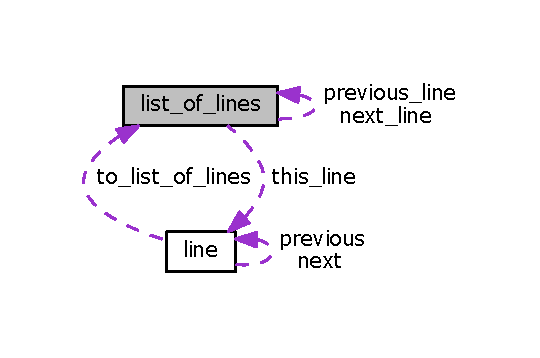
\includegraphics[width=259pt]{structlist__of__lines__coll__graph}
\end{center}
\end{figure}
\subsection*{Pola danych}
\begin{DoxyCompactItemize}
\item 
\hypertarget{structlist__of__lines_a7670f224d6f00d0198333a18f3f7c315}{struct \hyperlink{structlist__of__lines}{list\-\_\-of\-\_\-lines} $\ast$ \hyperlink{structlist__of__lines_a7670f224d6f00d0198333a18f3f7c315}{next\-\_\-line}}\label{structlist__of__lines_a7670f224d6f00d0198333a18f3f7c315}

\begin{DoxyCompactList}\small\item\em Indicator to next line in list of lines. \end{DoxyCompactList}\item 
\hypertarget{structlist__of__lines_a483118b9208361c9abaadd6c31c01b4f}{struct \hyperlink{structlist__of__lines}{list\-\_\-of\-\_\-lines} $\ast$ \hyperlink{structlist__of__lines_a483118b9208361c9abaadd6c31c01b4f}{previous\-\_\-line}}\label{structlist__of__lines_a483118b9208361c9abaadd6c31c01b4f}

\begin{DoxyCompactList}\small\item\em Indicator to previous line in list of lines. \end{DoxyCompactList}\item 
\hypertarget{structlist__of__lines_a3e9c87687a25f8afb98fe70ca294bd1c}{struct \hyperlink{structline}{line} $\ast$ \hyperlink{structlist__of__lines_a3e9c87687a25f8afb98fe70ca294bd1c}{this\-\_\-line}}\label{structlist__of__lines_a3e9c87687a25f8afb98fe70ca294bd1c}

\begin{DoxyCompactList}\small\item\em Indicator to fields in this line. \end{DoxyCompactList}\item 
\hypertarget{structlist__of__lines_a422664f6b1fecd50b43a0732624c3686}{int \hyperlink{structlist__of__lines_a422664f6b1fecd50b43a0732624c3686}{map\-\_\-size}}\label{structlist__of__lines_a422664f6b1fecd50b43a0732624c3686}

\begin{DoxyCompactList}\small\item\em Information about map\-\_\-size. \end{DoxyCompactList}\item 
\hypertarget{structlist__of__lines_a978838f8a1d0131c1273c2976d3e7bb8}{int \hyperlink{structlist__of__lines_a978838f8a1d0131c1273c2976d3e7bb8}{max\-\_\-number\-\_\-of\-\_\-turns}}\label{structlist__of__lines_a978838f8a1d0131c1273c2976d3e7bb8}

\begin{DoxyCompactList}\small\item\em Information about max\-\_\-number\-\_\-of\-\_\-turns. \end{DoxyCompactList}\item 
\hypertarget{structlist__of__lines_a6b2629df46fb4689e6b8ab3c20c7dfbd}{int \hyperlink{structlist__of__lines_a6b2629df46fb4689e6b8ab3c20c7dfbd}{number\-\_\-of\-\_\-line}}\label{structlist__of__lines_a6b2629df46fb4689e6b8ab3c20c7dfbd}

\begin{DoxyCompactList}\small\item\em Information about number\-\_\-of\-\_\-line. \end{DoxyCompactList}\end{DoxyCompactItemize}


\subsection{Opis szczegółowy}
Structure of \hyperlink{structlist__of__lines}{list\-\_\-of\-\_\-lines}. 

Dokumentacja dla tej struktury została wygenerowana z plików\-:\begin{DoxyCompactItemize}
\item 
engine.\-c\item 
\hyperlink{engine_8h}{engine.\-h}\end{DoxyCompactItemize}

\chapter{Dokumentacja plików}
\hypertarget{engine_8h}{\section{Dokumentacja pliku engine.\-h}
\label{engine_8h}\index{engine.\-h@{engine.\-h}}
}


Interface of game engine.  


Ten wykres pokazuje, które pliki bezpośrednio lub pośrednio załączają ten plik\-:\nopagebreak
\begin{figure}[H]
\begin{center}
\leavevmode
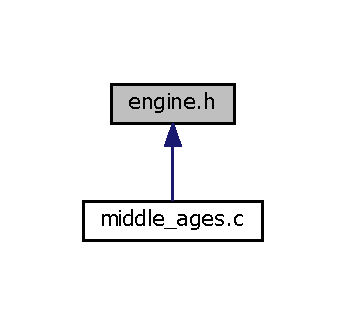
\includegraphics[width=166pt]{engine_8h__dep__incl}
\end{center}
\end{figure}
\subsection*{Struktury danych}
\begin{DoxyCompactItemize}
\item 
struct \hyperlink{structlist__of__lines}{list\-\_\-of\-\_\-lines}
\begin{DoxyCompactList}\small\item\em Structure of \hyperlink{structlist__of__lines}{list\-\_\-of\-\_\-lines}. \end{DoxyCompactList}\item 
struct \hyperlink{structline}{line}
\begin{DoxyCompactList}\small\item\em Structure of single line. \end{DoxyCompactList}\item 
struct \hyperlink{structinput__parameters}{input\-\_\-parameters}
\begin{DoxyCompactList}\small\item\em This structure include input parameters. \end{DoxyCompactList}\end{DoxyCompactItemize}
\subsection*{Definicje typów}
\begin{DoxyCompactItemize}
\item 
\hypertarget{engine_8h_a7bf8f2b3f2abed362e87e5156b0cad7d}{typedef struct \hyperlink{structlist__of__lines}{list\-\_\-of\-\_\-lines} \hyperlink{engine_8h_a7bf8f2b3f2abed362e87e5156b0cad7d}{type\-\_\-of\-\_\-list\-\_\-of\-\_\-lines}}\label{engine_8h_a7bf8f2b3f2abed362e87e5156b0cad7d}

\begin{DoxyCompactList}\small\item\em Structure of \hyperlink{structlist__of__lines}{list\-\_\-of\-\_\-lines}. \end{DoxyCompactList}\item 
\hypertarget{engine_8h_af61fc96585211a1dbb07a47db4abe8ca}{typedef struct \hyperlink{structline}{line} \hyperlink{engine_8h_af61fc96585211a1dbb07a47db4abe8ca}{type\-\_\-of\-\_\-line}}\label{engine_8h_af61fc96585211a1dbb07a47db4abe8ca}

\begin{DoxyCompactList}\small\item\em Structure of single line. \end{DoxyCompactList}\item 
\hypertarget{engine_8h_af248b9eb3c9bfb5ae6abeebc7c11fb60}{typedef struct \hyperlink{structinput__parameters}{input\-\_\-parameters} \hyperlink{engine_8h_af248b9eb3c9bfb5ae6abeebc7c11fb60}{type\-\_\-of\-\_\-input\-\_\-parameters}}\label{engine_8h_af248b9eb3c9bfb5ae6abeebc7c11fb60}

\begin{DoxyCompactList}\small\item\em This structure include input parameters. \end{DoxyCompactList}\end{DoxyCompactItemize}
\subsection*{Funkcje}
\begin{DoxyCompactItemize}
\item 
void \hyperlink{engine_8h_ab83db01d3f4a456157ab67717e594062}{make\-\_\-list\-\_\-empty} (\hyperlink{structlist__of__lines}{type\-\_\-of\-\_\-list\-\_\-of\-\_\-lines} $\ast$\hyperlink{engine_8h_a121e21e0e93b33f6071d24a43ce28830}{constructor\-\_\-of\-\_\-main\-\_\-list})
\begin{DoxyCompactList}\small\item\em This function makes main list empty, with no previous, and next field. \end{DoxyCompactList}\item 
void \hyperlink{engine_8h_a671b58f5509a3a9fa692bacccfc32cc9}{start\-\_\-game} ()
\begin{DoxyCompactList}\small\item\em Initializes a game. \end{DoxyCompactList}\item 
void \hyperlink{engine_8h_a4202fa5c5191c7e387d7570da6c8cd8c}{end\-\_\-game} ()
\begin{DoxyCompactList}\small\item\em Frees memory. \end{DoxyCompactList}\item 
void \hyperlink{engine_8h_a04919bedca6c747ff007c23783d37d28}{incorrect\-\_\-command} ()
\begin{DoxyCompactList}\small\item\em This function enforce incorrect command with exit(42) result. \end{DoxyCompactList}\item 
void \hyperlink{engine_8h_a61500581d49ed801deeaa1b0e1c4710d}{print\-\_\-symbol} (\hyperlink{structline}{type\-\_\-of\-\_\-line} $\ast$iterator\-\_\-on\-\_\-line)
\begin{DoxyCompactList}\small\item\em This function print symbol of given field. \end{DoxyCompactList}\item 
void \hyperlink{engine_8h_a6351fcf47fb1cd042b83da768706e567}{print\-\_\-empty\-\_\-line} (int size\-\_\-to\-\_\-print)
\begin{DoxyCompactList}\small\item\em This function print empty line (line full of spaces) which include given amount of spaces. \end{DoxyCompactList}\item 
void \hyperlink{engine_8h_a1fb95c1cfdb44f81d4ba80658b50913d}{print\-\_\-topleft} ()
\begin{DoxyCompactList}\small\item\em Prints (into stdout) top-\/left corner of the board of size m x m where m = min(n,10). \end{DoxyCompactList}\item 
void \hyperlink{engine_8h_aeb8e3f2cbbdfb88436ca9d4a3459470c}{create\-\_\-character} (\hyperlink{structline}{type\-\_\-of\-\_\-line} $\ast$character, int x)
\begin{DoxyCompactList}\small\item\em This function create peasant for init. \end{DoxyCompactList}\item 
void \hyperlink{engine_8h_a320f52edf861f22d744f24cd9d8999a7}{create\-\_\-king} (\hyperlink{structline}{type\-\_\-of\-\_\-line} $\ast$king, int x)
\begin{DoxyCompactList}\small\item\em This function create peasant for init needs using create\-\_\-character function. \end{DoxyCompactList}\item 
void \hyperlink{engine_8h_a9437c65c740ed267afb70ac58b1a3b22}{create\-\_\-knight} (\hyperlink{structline}{type\-\_\-of\-\_\-line} $\ast$knight, int x)
\begin{DoxyCompactList}\small\item\em This function create knight for init needs using create\-\_\-character function. \end{DoxyCompactList}\item 
void \hyperlink{engine_8h_a298684de9430c77f30583d99098780b5}{create\-\_\-peasant} (\hyperlink{structline}{type\-\_\-of\-\_\-line} $\ast$peasant, int x)
\begin{DoxyCompactList}\small\item\em This function create peasant for init needs using create\-\_\-character function. \end{DoxyCompactList}\item 
void \hyperlink{engine_8h_a356d8f07535e1016fbe5a6fdddb33516}{put\-\_\-in\-\_\-line} (\hyperlink{structline}{type\-\_\-of\-\_\-line} $\ast$new\-\_\-line1, \hyperlink{structline}{type\-\_\-of\-\_\-line} $\ast$king, \hyperlink{structline}{type\-\_\-of\-\_\-line} $\ast$peasant, \hyperlink{structline}{type\-\_\-of\-\_\-line} $\ast$knight1, \hyperlink{structline}{type\-\_\-of\-\_\-line} $\ast$knight2)
\begin{DoxyCompactList}\small\item\em This function put king, peasant, knight1 and knigth2 to line behind new\-\_\-line1. \end{DoxyCompactList}\item 
void \hyperlink{engine_8h_af0e24474a4a8addf53dba7a206ad572d}{create\-\_\-line} (\hyperlink{structlist__of__lines}{type\-\_\-of\-\_\-list\-\_\-of\-\_\-lines} $\ast$new\-\_\-line, int y)
\begin{DoxyCompactList}\small\item\em This function create mock for new\-\_\-line and set pos\-\_\-x of this mock on (-\/1). \end{DoxyCompactList}\item 
int \hyperlink{engine_8h_a9be3a11fc5243aaf3d38b22e1645ada2}{absolute\-\_\-value} (int number)
\begin{DoxyCompactList}\small\item\em This function return absolute value of given number. \end{DoxyCompactList}\item 
void \hyperlink{engine_8h_ae4e387369a6f703ef76b1c328a5b7f41}{check\-\_\-correctness\-\_\-of\-\_\-input} (int n, int k, int p, int x1, int y1, int x2, int y2)
\begin{DoxyCompactList}\small\item\em This function check if input is correct. \end{DoxyCompactList}\item 
void \hyperlink{engine_8h_a5a05a64cb2e0a004c78d0067fa4af905}{check\-\_\-correctness\-\_\-of\-\_\-positions\-\_\-to\-\_\-move\-\_\-or\-\_\-produce} (int x1, int y1, int x2, int y2)
\begin{DoxyCompactList}\small\item\em This function check if positions are correct to make action. \end{DoxyCompactList}\item 
void \hyperlink{engine_8h_a8e474b14265a2ebbcb0c7461817214bc}{set\-\_\-input\-\_\-parameters} (int n, int k, int p, int x1, int y1, int x2, int y2)
\begin{DoxyCompactList}\small\item\em This function memorize parameters given with I\-N\-I\-T. \end{DoxyCompactList}\item 
void \hyperlink{engine_8h_a512751eb67e971e92a205e39ee8dfe57}{init} (int n, int k, int p, int x1, int y1, int x2, int y2)
\begin{DoxyCompactList}\small\item\em Initializes a game with size of a board, number of rounds and positions of kings. \end{DoxyCompactList}\item 
\hypertarget{engine_8h_a99cab52e7cfcf0e6ff4808ce3f6a74b1}{\hyperlink{structlist__of__lines}{type\-\_\-of\-\_\-list\-\_\-of\-\_\-lines} $\ast$ \hyperlink{engine_8h_a99cab52e7cfcf0e6ff4808ce3f6a74b1}{find\-\_\-line} (int y)}\label{engine_8h_a99cab52e7cfcf0e6ff4808ce3f6a74b1}

\begin{DoxyCompactList}\small\item\em This function look for line with index y. \end{DoxyCompactList}\item 
\hyperlink{structline}{type\-\_\-of\-\_\-line} $\ast$ \hyperlink{engine_8h_a548fff34b91e10f9ff3779c15a10ef93}{find\-\_\-field} (\hyperlink{structlist__of__lines}{type\-\_\-of\-\_\-list\-\_\-of\-\_\-lines} $\ast$iterator, int x)
\begin{DoxyCompactList}\small\item\em This function look for field with index x, in the given line. \end{DoxyCompactList}\item 
void \hyperlink{engine_8h_afc70ff78ef5f19df54275f66f91e10b2}{delete\-\_\-field} (\hyperlink{structline}{type\-\_\-of\-\_\-line} $\ast$character)
\begin{DoxyCompactList}\small\item\em This function delete given field and if it was last field delete whole line. \end{DoxyCompactList}\item 
\hypertarget{engine_8h_a56c5cf8a568cff737ff95520cbe6b405}{void \hyperlink{engine_8h_a56c5cf8a568cff737ff95520cbe6b405}{draw} ()}\label{engine_8h_a56c5cf8a568cff737ff95520cbe6b405}

\begin{DoxyCompactList}\small\item\em This function end game with draw result. \end{DoxyCompactList}\item 
void \hyperlink{engine_8h_a32951a11c14553f0e03ed2e7576f2748}{player\-\_\-won} (int \hyperlink{engine_8h_a230bf1ce6f1480f9fddb4577d1742f4f}{player\-\_\-number})
\begin{DoxyCompactList}\small\item\em This function end game with win result of one of players. \end{DoxyCompactList}\item 
void \hyperlink{engine_8h_a31d63d997d23cb4de7d589f0f8a5b337}{fight} (\hyperlink{structline}{type\-\_\-of\-\_\-line} $\ast$character1, \hyperlink{structline}{type\-\_\-of\-\_\-line} $\ast$character2)
\begin{DoxyCompactList}\small\item\em This function make fight between character1 and character2 and delete fields killed characters. \end{DoxyCompactList}\item 
void \hyperlink{engine_8h_a19b6e533c5b9bde71c3c38e571b0917b}{clone\-\_\-field} (\hyperlink{structline}{type\-\_\-of\-\_\-line} $\ast$field, \hyperlink{structline}{type\-\_\-of\-\_\-line} $\ast$new\-\_\-field)
\begin{DoxyCompactList}\small\item\em This function copy every parameters from field to new\-\_\-field. \end{DoxyCompactList}\item 
void \hyperlink{engine_8h_a484a4ab3480af45c873b3333f0cacee1}{move} (int x1, int y1, int x2, int y2)
\begin{DoxyCompactList}\small\item\em This function move characters from place coordinates (x1, y1) to (x2, y2) if it is possible. \end{DoxyCompactList}\item 
\hyperlink{structline}{type\-\_\-of\-\_\-line} $\ast$ \hyperlink{engine_8h_a33a2165cf3d1a1dbfed5422b2226a0d7}{produce\-\_\-unit} (int x1, int y1, int x2, int y2)
\begin{DoxyCompactList}\small\item\em This function results in production unit on field with coordinates (x2, y2) by peasant on field with coordinates (x1, y1) \end{DoxyCompactList}\item 
void \hyperlink{engine_8h_ab6b332d9aad7c1d874fa9ca3c8e13d05}{produce\-\_\-knight} (int x1, int y1, int x2, int y2)
\begin{DoxyCompactList}\small\item\em This function produce unit using produce\-\_\-unit(x1, y1, x2, y2) function and give to this unit knight attribute. \end{DoxyCompactList}\item 
void \hyperlink{engine_8h_abb4d3708d6bdc644d179a3630518a2b2}{produce\-\_\-peasant} (int x1, int y1, int x2, int y2)
\begin{DoxyCompactList}\small\item\em This function produce unit using produce\-\_\-unit(x1, y1, x2, y2) function and give to this unit peasant attribute. \end{DoxyCompactList}\item 
void \hyperlink{engine_8h_a6c355efb3996f6ddcc16c27d0224bfb0}{end\-\_\-turn} ()
\begin{DoxyCompactList}\small\item\em This function end turn of one of players, and check if the number of played turns isn't bigger than max\-\_\-number\-\_\-of\-\_\-turns. \end{DoxyCompactList}\end{DoxyCompactItemize}
\subsection*{Zmienne}
\begin{DoxyCompactItemize}
\item 
\hyperlink{structlist__of__lines}{type\-\_\-of\-\_\-list\-\_\-of\-\_\-lines} $\ast$ \hyperlink{engine_8h_a121e21e0e93b33f6071d24a43ce28830}{constructor\-\_\-of\-\_\-main\-\_\-list}
\begin{DoxyCompactList}\small\item\em Pointer to mock of list of lines. \end{DoxyCompactList}\item 
\hyperlink{structinput__parameters}{type\-\_\-of\-\_\-input\-\_\-parameters} \hyperlink{engine_8h_aad242164bb0908170880af0688ed3438}{input}
\begin{DoxyCompactList}\small\item\em Memory of input parameters. \end{DoxyCompactList}\item 
int \hyperlink{engine_8h_ac04a3e0434907c4977d4cc8592472e4e}{number\-\_\-of\-\_\-init}
\begin{DoxyCompactList}\small\item\em Counter of number of initializations. \end{DoxyCompactList}\item 
int \hyperlink{engine_8h_a230bf1ce6f1480f9fddb4577d1742f4f}{player\-\_\-number}
\begin{DoxyCompactList}\small\item\em Counter of actually playing player. \end{DoxyCompactList}\item 
int \hyperlink{engine_8h_aa60bf4b5b108d9591140a5abfc89c5fb}{counter\-\_\-of\-\_\-rounds}
\begin{DoxyCompactList}\small\item\em Counter of actually playing turn. \end{DoxyCompactList}\end{DoxyCompactItemize}


\subsection{Opis szczegółowy}
Interface of game engine. 

\subsection{Dokumentacja funkcji}
\hypertarget{engine_8h_a9be3a11fc5243aaf3d38b22e1645ada2}{\index{engine.\-h@{engine.\-h}!absolute\-\_\-value@{absolute\-\_\-value}}
\index{absolute\-\_\-value@{absolute\-\_\-value}!engine.h@{engine.\-h}}
\subsubsection[{absolute\-\_\-value}]{\setlength{\rightskip}{0pt plus 5cm}int absolute\-\_\-value (
\begin{DoxyParamCaption}
\item[{int}]{number}
\end{DoxyParamCaption}
)}}\label{engine_8h_a9be3a11fc5243aaf3d38b22e1645ada2}


This function return absolute value of given number. 



Oto graf wywoływań tej funkcji\-:\nopagebreak
\begin{figure}[H]
\begin{center}
\leavevmode
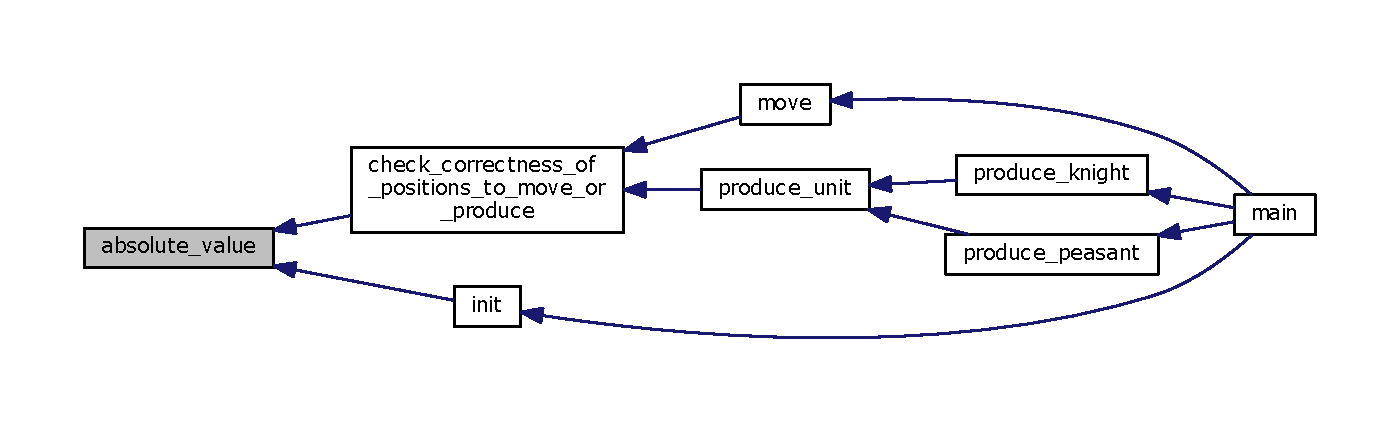
\includegraphics[width=350pt]{engine_8h_a9be3a11fc5243aaf3d38b22e1645ada2_icgraph}
\end{center}
\end{figure}


\hypertarget{engine_8h_ae4e387369a6f703ef76b1c328a5b7f41}{\index{engine.\-h@{engine.\-h}!check\-\_\-correctness\-\_\-of\-\_\-input@{check\-\_\-correctness\-\_\-of\-\_\-input}}
\index{check\-\_\-correctness\-\_\-of\-\_\-input@{check\-\_\-correctness\-\_\-of\-\_\-input}!engine.h@{engine.\-h}}
\subsubsection[{check\-\_\-correctness\-\_\-of\-\_\-input}]{\setlength{\rightskip}{0pt plus 5cm}void check\-\_\-correctness\-\_\-of\-\_\-input (
\begin{DoxyParamCaption}
\item[{int}]{n, }
\item[{int}]{k, }
\item[{int}]{p, }
\item[{int}]{x1, }
\item[{int}]{y1, }
\item[{int}]{x2, }
\item[{int}]{y2}
\end{DoxyParamCaption}
)}}\label{engine_8h_ae4e387369a6f703ef76b1c328a5b7f41}


This function check if input is correct. 



Oto graf wywołań dla tej funkcji\-:\nopagebreak
\begin{figure}[H]
\begin{center}
\leavevmode
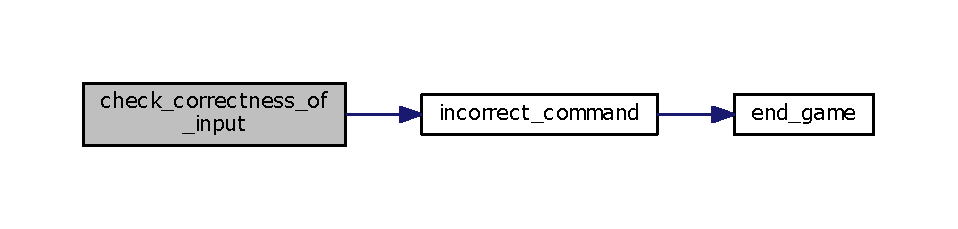
\includegraphics[width=350pt]{engine_8h_ae4e387369a6f703ef76b1c328a5b7f41_cgraph}
\end{center}
\end{figure}




Oto graf wywoływań tej funkcji\-:\nopagebreak
\begin{figure}[H]
\begin{center}
\leavevmode
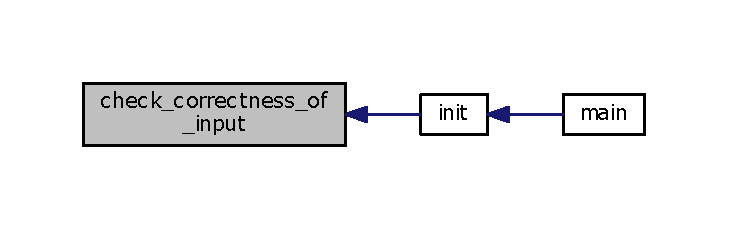
\includegraphics[width=350pt]{engine_8h_ae4e387369a6f703ef76b1c328a5b7f41_icgraph}
\end{center}
\end{figure}


\hypertarget{engine_8h_a5a05a64cb2e0a004c78d0067fa4af905}{\index{engine.\-h@{engine.\-h}!check\-\_\-correctness\-\_\-of\-\_\-positions\-\_\-to\-\_\-move\-\_\-or\-\_\-produce@{check\-\_\-correctness\-\_\-of\-\_\-positions\-\_\-to\-\_\-move\-\_\-or\-\_\-produce}}
\index{check\-\_\-correctness\-\_\-of\-\_\-positions\-\_\-to\-\_\-move\-\_\-or\-\_\-produce@{check\-\_\-correctness\-\_\-of\-\_\-positions\-\_\-to\-\_\-move\-\_\-or\-\_\-produce}!engine.h@{engine.\-h}}
\subsubsection[{check\-\_\-correctness\-\_\-of\-\_\-positions\-\_\-to\-\_\-move\-\_\-or\-\_\-produce}]{\setlength{\rightskip}{0pt plus 5cm}void check\-\_\-correctness\-\_\-of\-\_\-positions\-\_\-to\-\_\-move\-\_\-or\-\_\-produce (
\begin{DoxyParamCaption}
\item[{int}]{x1, }
\item[{int}]{y1, }
\item[{int}]{x2, }
\item[{int}]{y2}
\end{DoxyParamCaption}
)}}\label{engine_8h_a5a05a64cb2e0a004c78d0067fa4af905}


This function check if positions are correct to make action. 



Oto graf wywołań dla tej funkcji\-:\nopagebreak
\begin{figure}[H]
\begin{center}
\leavevmode
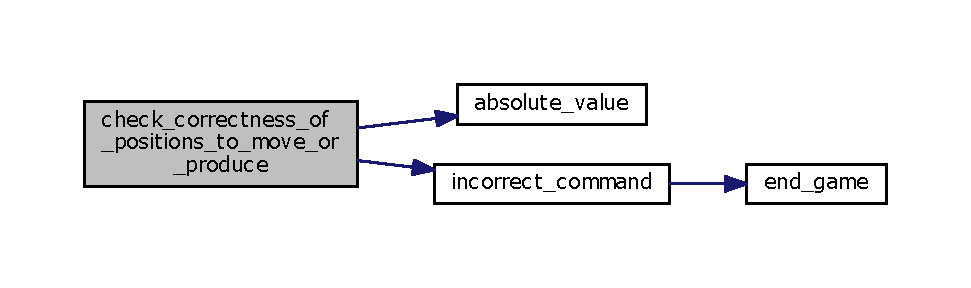
\includegraphics[width=350pt]{engine_8h_a5a05a64cb2e0a004c78d0067fa4af905_cgraph}
\end{center}
\end{figure}




Oto graf wywoływań tej funkcji\-:\nopagebreak
\begin{figure}[H]
\begin{center}
\leavevmode
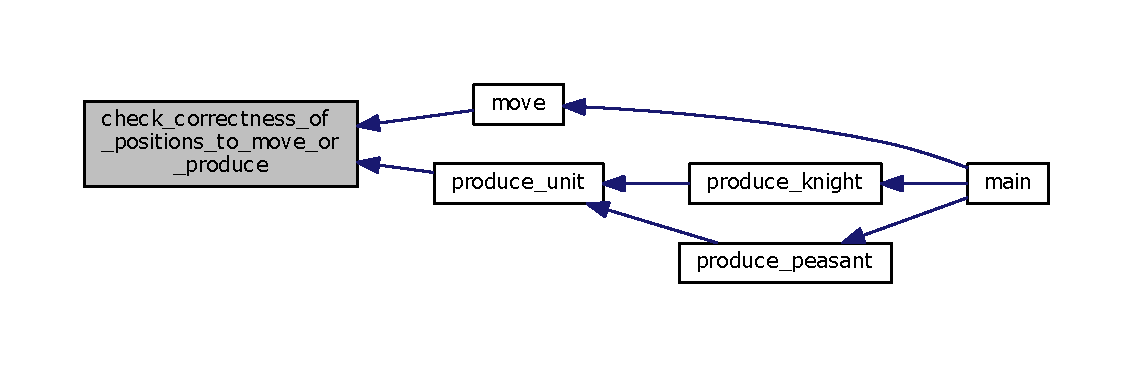
\includegraphics[width=350pt]{engine_8h_a5a05a64cb2e0a004c78d0067fa4af905_icgraph}
\end{center}
\end{figure}


\hypertarget{engine_8h_a19b6e533c5b9bde71c3c38e571b0917b}{\index{engine.\-h@{engine.\-h}!clone\-\_\-field@{clone\-\_\-field}}
\index{clone\-\_\-field@{clone\-\_\-field}!engine.h@{engine.\-h}}
\subsubsection[{clone\-\_\-field}]{\setlength{\rightskip}{0pt plus 5cm}void clone\-\_\-field (
\begin{DoxyParamCaption}
\item[{{\bf type\-\_\-of\-\_\-line} $\ast$}]{field, }
\item[{{\bf type\-\_\-of\-\_\-line} $\ast$}]{new\-\_\-field}
\end{DoxyParamCaption}
)}}\label{engine_8h_a19b6e533c5b9bde71c3c38e571b0917b}


This function copy every parameters from field to new\-\_\-field. 


\begin{DoxyParams}[1]{Parametry}
\mbox{\tt in}  & {\em field} & Field with parameters which we copy. \\
\hline
\mbox{\tt in}  & {\em new\-\_\-field} & Field which receive copied parameters. \\
\hline
\end{DoxyParams}


Oto graf wywoływań tej funkcji\-:\nopagebreak
\begin{figure}[H]
\begin{center}
\leavevmode
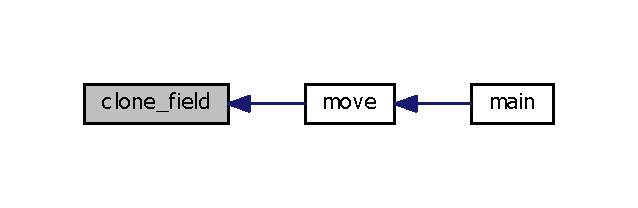
\includegraphics[width=306pt]{engine_8h_a19b6e533c5b9bde71c3c38e571b0917b_icgraph}
\end{center}
\end{figure}


\hypertarget{engine_8h_aeb8e3f2cbbdfb88436ca9d4a3459470c}{\index{engine.\-h@{engine.\-h}!create\-\_\-character@{create\-\_\-character}}
\index{create\-\_\-character@{create\-\_\-character}!engine.h@{engine.\-h}}
\subsubsection[{create\-\_\-character}]{\setlength{\rightskip}{0pt plus 5cm}void create\-\_\-character (
\begin{DoxyParamCaption}
\item[{{\bf type\-\_\-of\-\_\-line} $\ast$}]{character, }
\item[{int}]{x}
\end{DoxyParamCaption}
)}}\label{engine_8h_aeb8e3f2cbbdfb88436ca9d4a3459470c}


This function create peasant for init. 


\begin{DoxyParams}[1]{Parametry}
\mbox{\tt in}  & {\em character} & Indicator to field of created character. \\
\hline
\mbox{\tt in}  & {\em x} & X-\/\-Coordinate of created character. \\
\hline
\end{DoxyParams}


Oto graf wywoływań tej funkcji\-:\nopagebreak
\begin{figure}[H]
\begin{center}
\leavevmode
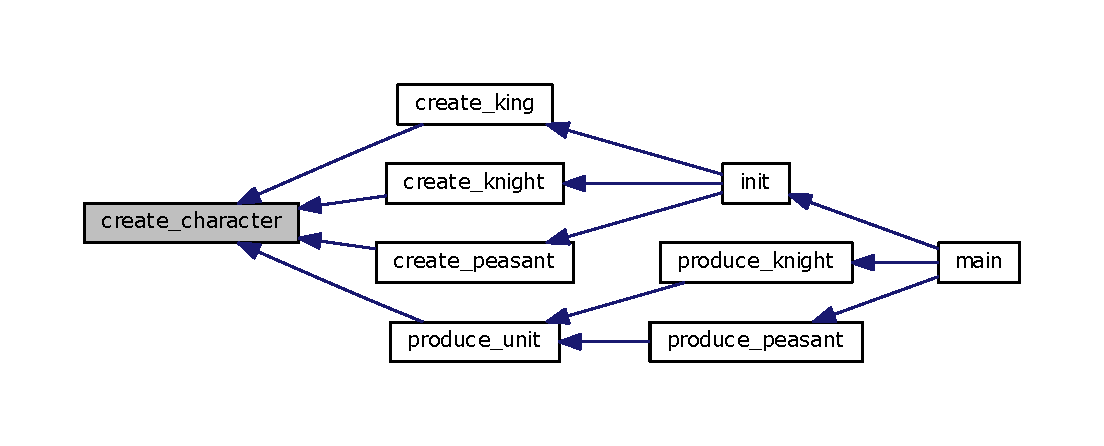
\includegraphics[width=350pt]{engine_8h_aeb8e3f2cbbdfb88436ca9d4a3459470c_icgraph}
\end{center}
\end{figure}


\hypertarget{engine_8h_a320f52edf861f22d744f24cd9d8999a7}{\index{engine.\-h@{engine.\-h}!create\-\_\-king@{create\-\_\-king}}
\index{create\-\_\-king@{create\-\_\-king}!engine.h@{engine.\-h}}
\subsubsection[{create\-\_\-king}]{\setlength{\rightskip}{0pt plus 5cm}void create\-\_\-king (
\begin{DoxyParamCaption}
\item[{{\bf type\-\_\-of\-\_\-line} $\ast$}]{king, }
\item[{int}]{x}
\end{DoxyParamCaption}
)}}\label{engine_8h_a320f52edf861f22d744f24cd9d8999a7}


This function create peasant for init needs using create\-\_\-character function. 


\begin{DoxyParams}[1]{Parametry}
\mbox{\tt in}  & {\em king} & Indicator to field of created king. \\
\hline
\mbox{\tt in}  & {\em x} & X-\/\-Coordinate of created king. \\
\hline
\end{DoxyParams}


Oto graf wywołań dla tej funkcji\-:\nopagebreak
\begin{figure}[H]
\begin{center}
\leavevmode
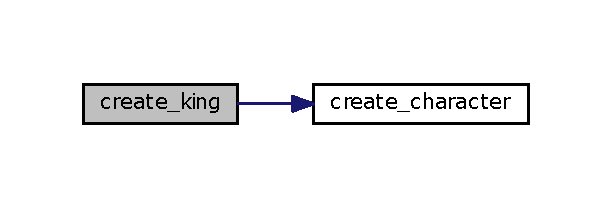
\includegraphics[width=294pt]{engine_8h_a320f52edf861f22d744f24cd9d8999a7_cgraph}
\end{center}
\end{figure}




Oto graf wywoływań tej funkcji\-:\nopagebreak
\begin{figure}[H]
\begin{center}
\leavevmode
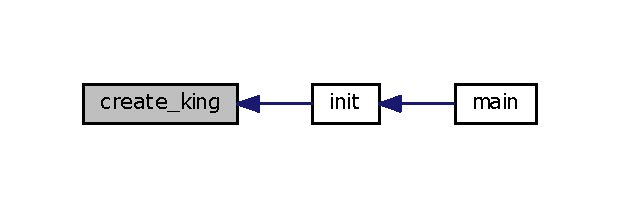
\includegraphics[width=298pt]{engine_8h_a320f52edf861f22d744f24cd9d8999a7_icgraph}
\end{center}
\end{figure}


\hypertarget{engine_8h_a9437c65c740ed267afb70ac58b1a3b22}{\index{engine.\-h@{engine.\-h}!create\-\_\-knight@{create\-\_\-knight}}
\index{create\-\_\-knight@{create\-\_\-knight}!engine.h@{engine.\-h}}
\subsubsection[{create\-\_\-knight}]{\setlength{\rightskip}{0pt plus 5cm}void create\-\_\-knight (
\begin{DoxyParamCaption}
\item[{{\bf type\-\_\-of\-\_\-line} $\ast$}]{knight, }
\item[{int}]{x}
\end{DoxyParamCaption}
)}}\label{engine_8h_a9437c65c740ed267afb70ac58b1a3b22}


This function create knight for init needs using create\-\_\-character function. 


\begin{DoxyParams}[1]{Parametry}
\mbox{\tt in}  & {\em knight} & Indicator to field of created knight. \\
\hline
\mbox{\tt in}  & {\em x} & X-\/\-Coordinate of created knight. \\
\hline
\end{DoxyParams}


Oto graf wywołań dla tej funkcji\-:\nopagebreak
\begin{figure}[H]
\begin{center}
\leavevmode
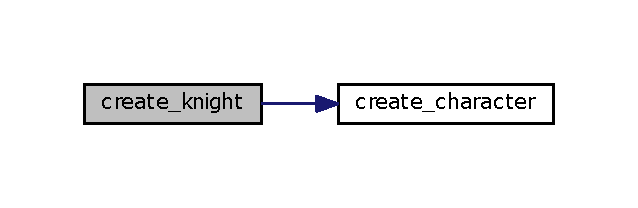
\includegraphics[width=306pt]{engine_8h_a9437c65c740ed267afb70ac58b1a3b22_cgraph}
\end{center}
\end{figure}




Oto graf wywoływań tej funkcji\-:\nopagebreak
\begin{figure}[H]
\begin{center}
\leavevmode
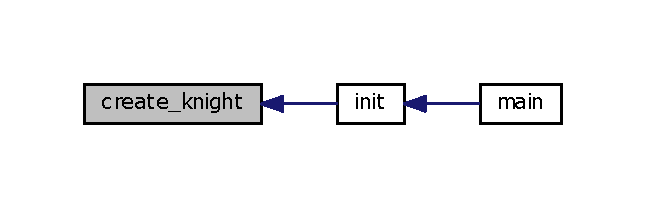
\includegraphics[width=310pt]{engine_8h_a9437c65c740ed267afb70ac58b1a3b22_icgraph}
\end{center}
\end{figure}


\hypertarget{engine_8h_af0e24474a4a8addf53dba7a206ad572d}{\index{engine.\-h@{engine.\-h}!create\-\_\-line@{create\-\_\-line}}
\index{create\-\_\-line@{create\-\_\-line}!engine.h@{engine.\-h}}
\subsubsection[{create\-\_\-line}]{\setlength{\rightskip}{0pt plus 5cm}void create\-\_\-line (
\begin{DoxyParamCaption}
\item[{{\bf type\-\_\-of\-\_\-list\-\_\-of\-\_\-lines} $\ast$}]{new\-\_\-line, }
\item[{int}]{y}
\end{DoxyParamCaption}
)}}\label{engine_8h_af0e24474a4a8addf53dba7a206ad572d}


This function create mock for new\-\_\-line and set pos\-\_\-x of this mock on (-\/1). 



Oto graf wywoływań tej funkcji\-:\nopagebreak
\begin{figure}[H]
\begin{center}
\leavevmode
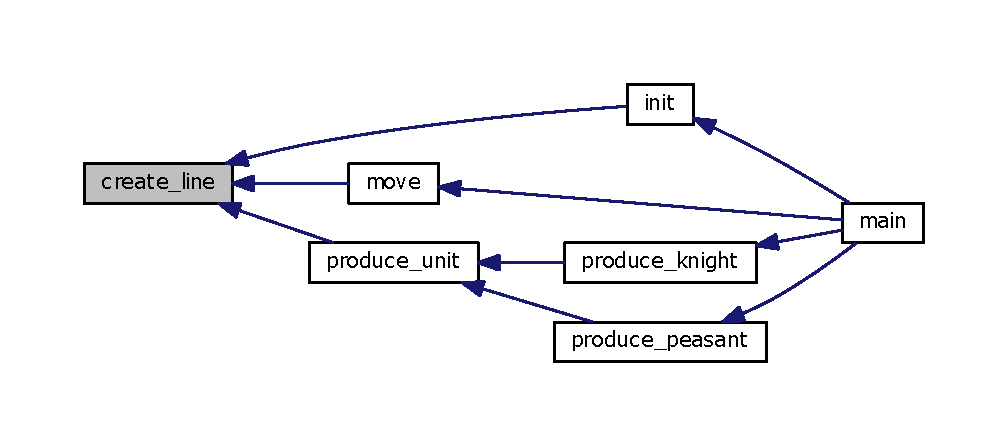
\includegraphics[width=350pt]{engine_8h_af0e24474a4a8addf53dba7a206ad572d_icgraph}
\end{center}
\end{figure}


\hypertarget{engine_8h_a298684de9430c77f30583d99098780b5}{\index{engine.\-h@{engine.\-h}!create\-\_\-peasant@{create\-\_\-peasant}}
\index{create\-\_\-peasant@{create\-\_\-peasant}!engine.h@{engine.\-h}}
\subsubsection[{create\-\_\-peasant}]{\setlength{\rightskip}{0pt plus 5cm}void create\-\_\-peasant (
\begin{DoxyParamCaption}
\item[{{\bf type\-\_\-of\-\_\-line} $\ast$}]{peasant, }
\item[{int}]{x}
\end{DoxyParamCaption}
)}}\label{engine_8h_a298684de9430c77f30583d99098780b5}


This function create peasant for init needs using create\-\_\-character function. 


\begin{DoxyParams}[1]{Parametry}
\mbox{\tt in}  & {\em peasant} & Indicator to field of created peasant. \\
\hline
\mbox{\tt in}  & {\em x} & X-\/\-Coordinate of created peasant. \\
\hline
\end{DoxyParams}


Oto graf wywołań dla tej funkcji\-:\nopagebreak
\begin{figure}[H]
\begin{center}
\leavevmode
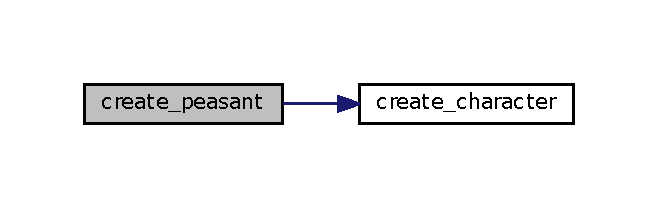
\includegraphics[width=316pt]{engine_8h_a298684de9430c77f30583d99098780b5_cgraph}
\end{center}
\end{figure}




Oto graf wywoływań tej funkcji\-:\nopagebreak
\begin{figure}[H]
\begin{center}
\leavevmode
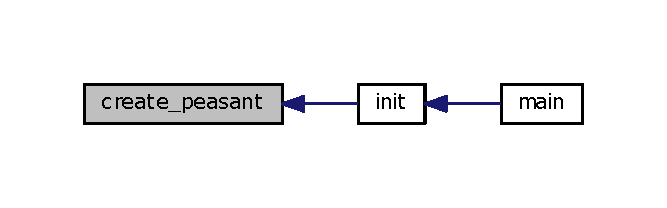
\includegraphics[width=320pt]{engine_8h_a298684de9430c77f30583d99098780b5_icgraph}
\end{center}
\end{figure}


\hypertarget{engine_8h_afc70ff78ef5f19df54275f66f91e10b2}{\index{engine.\-h@{engine.\-h}!delete\-\_\-field@{delete\-\_\-field}}
\index{delete\-\_\-field@{delete\-\_\-field}!engine.h@{engine.\-h}}
\subsubsection[{delete\-\_\-field}]{\setlength{\rightskip}{0pt plus 5cm}void delete\-\_\-field (
\begin{DoxyParamCaption}
\item[{{\bf type\-\_\-of\-\_\-line} $\ast$}]{character}
\end{DoxyParamCaption}
)}}\label{engine_8h_afc70ff78ef5f19df54275f66f91e10b2}


This function delete given field and if it was last field delete whole line. 


\begin{DoxyParams}[1]{Parametry}
\mbox{\tt in}  & {\em character} & Field which will be delete \\
\hline
\end{DoxyParams}


Oto graf wywoływań tej funkcji\-:\nopagebreak
\begin{figure}[H]
\begin{center}
\leavevmode
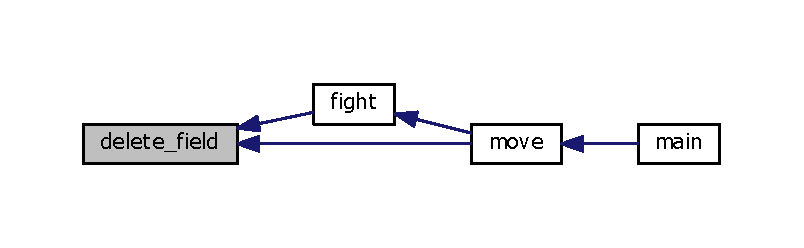
\includegraphics[width=350pt]{engine_8h_afc70ff78ef5f19df54275f66f91e10b2_icgraph}
\end{center}
\end{figure}


\hypertarget{engine_8h_a4202fa5c5191c7e387d7570da6c8cd8c}{\index{engine.\-h@{engine.\-h}!end\-\_\-game@{end\-\_\-game}}
\index{end\-\_\-game@{end\-\_\-game}!engine.h@{engine.\-h}}
\subsubsection[{end\-\_\-game}]{\setlength{\rightskip}{0pt plus 5cm}void end\-\_\-game (
\begin{DoxyParamCaption}
{}
\end{DoxyParamCaption}
)}}\label{engine_8h_a4202fa5c5191c7e387d7570da6c8cd8c}


Frees memory. 

Needed after finishing game. 

Oto graf wywoływań tej funkcji\-:\nopagebreak
\begin{figure}[H]
\begin{center}
\leavevmode
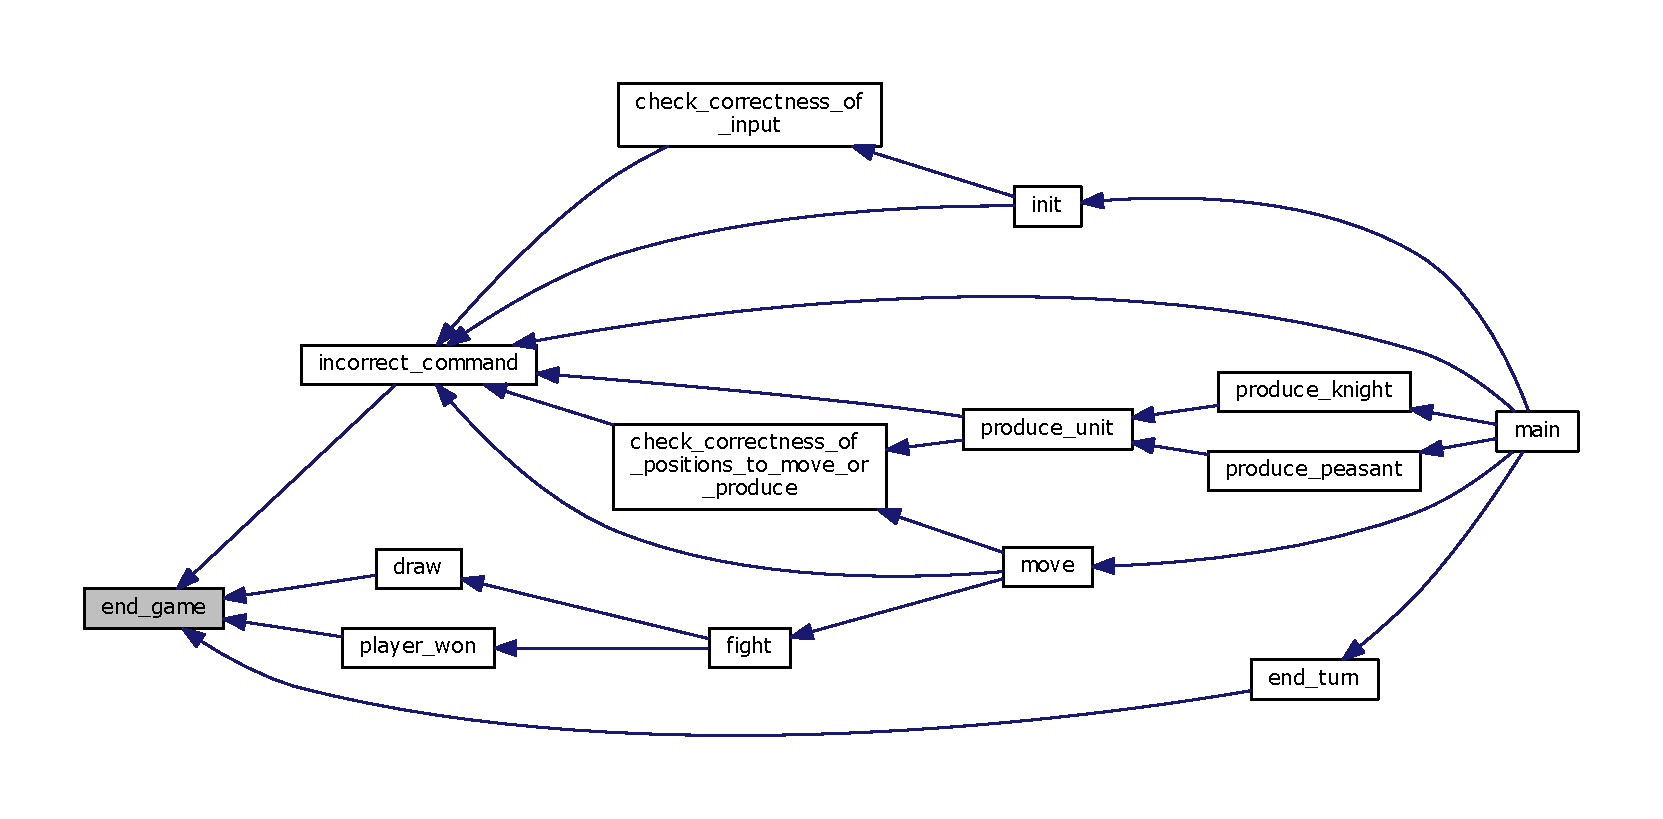
\includegraphics[width=350pt]{engine_8h_a4202fa5c5191c7e387d7570da6c8cd8c_icgraph}
\end{center}
\end{figure}


\hypertarget{engine_8h_a6c355efb3996f6ddcc16c27d0224bfb0}{\index{engine.\-h@{engine.\-h}!end\-\_\-turn@{end\-\_\-turn}}
\index{end\-\_\-turn@{end\-\_\-turn}!engine.h@{engine.\-h}}
\subsubsection[{end\-\_\-turn}]{\setlength{\rightskip}{0pt plus 5cm}void end\-\_\-turn (
\begin{DoxyParamCaption}
{}
\end{DoxyParamCaption}
)}}\label{engine_8h_a6c355efb3996f6ddcc16c27d0224bfb0}


This function end turn of one of players, and check if the number of played turns isn't bigger than max\-\_\-number\-\_\-of\-\_\-turns. 



Oto graf wywołań dla tej funkcji\-:\nopagebreak
\begin{figure}[H]
\begin{center}
\leavevmode
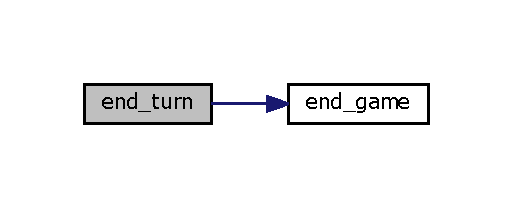
\includegraphics[width=246pt]{engine_8h_a6c355efb3996f6ddcc16c27d0224bfb0_cgraph}
\end{center}
\end{figure}




Oto graf wywoływań tej funkcji\-:\nopagebreak
\begin{figure}[H]
\begin{center}
\leavevmode
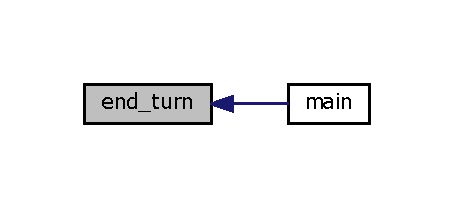
\includegraphics[width=218pt]{engine_8h_a6c355efb3996f6ddcc16c27d0224bfb0_icgraph}
\end{center}
\end{figure}


\hypertarget{engine_8h_a31d63d997d23cb4de7d589f0f8a5b337}{\index{engine.\-h@{engine.\-h}!fight@{fight}}
\index{fight@{fight}!engine.h@{engine.\-h}}
\subsubsection[{fight}]{\setlength{\rightskip}{0pt plus 5cm}void fight (
\begin{DoxyParamCaption}
\item[{{\bf type\-\_\-of\-\_\-line} $\ast$}]{character1, }
\item[{{\bf type\-\_\-of\-\_\-line} $\ast$}]{character2}
\end{DoxyParamCaption}
)}}\label{engine_8h_a31d63d997d23cb4de7d589f0f8a5b337}


This function make fight between character1 and character2 and delete fields killed characters. 


\begin{DoxyParams}[1]{Parametry}
\mbox{\tt in}  & {\em character1} & Participant of fight. \\
\hline
\mbox{\tt in}  & {\em character2} & Participant of fight. \\
\hline
\end{DoxyParams}


Oto graf wywołań dla tej funkcji\-:\nopagebreak
\begin{figure}[H]
\begin{center}
\leavevmode
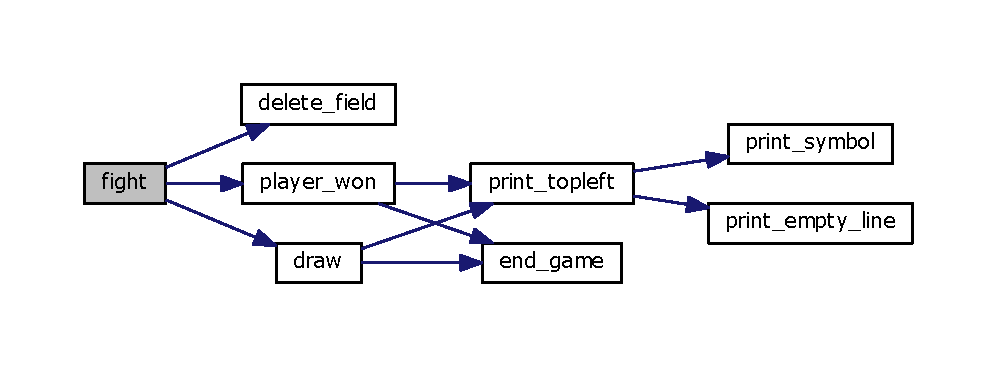
\includegraphics[width=350pt]{engine_8h_a31d63d997d23cb4de7d589f0f8a5b337_cgraph}
\end{center}
\end{figure}




Oto graf wywoływań tej funkcji\-:\nopagebreak
\begin{figure}[H]
\begin{center}
\leavevmode
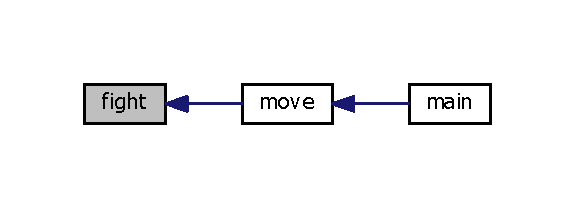
\includegraphics[width=276pt]{engine_8h_a31d63d997d23cb4de7d589f0f8a5b337_icgraph}
\end{center}
\end{figure}


\hypertarget{engine_8h_a548fff34b91e10f9ff3779c15a10ef93}{\index{engine.\-h@{engine.\-h}!find\-\_\-field@{find\-\_\-field}}
\index{find\-\_\-field@{find\-\_\-field}!engine.h@{engine.\-h}}
\subsubsection[{find\-\_\-field}]{\setlength{\rightskip}{0pt plus 5cm}{\bf type\-\_\-of\-\_\-line}$\ast$ find\-\_\-field (
\begin{DoxyParamCaption}
\item[{{\bf type\-\_\-of\-\_\-list\-\_\-of\-\_\-lines} $\ast$}]{iterator, }
\item[{int}]{x}
\end{DoxyParamCaption}
)}}\label{engine_8h_a548fff34b91e10f9ff3779c15a10ef93}


This function look for field with index x, in the given line. 


\begin{DoxyParams}[1]{Parametry}
\mbox{\tt in}  & {\em iterator} & Pointer to line where function looks for field with X-\/\-Coordinate = x. \\
\hline
\mbox{\tt in}  & {\em x} & X-\/\-Coordinate of searches field. \\
\hline
\end{DoxyParams}


Oto graf wywoływań tej funkcji\-:\nopagebreak
\begin{figure}[H]
\begin{center}
\leavevmode
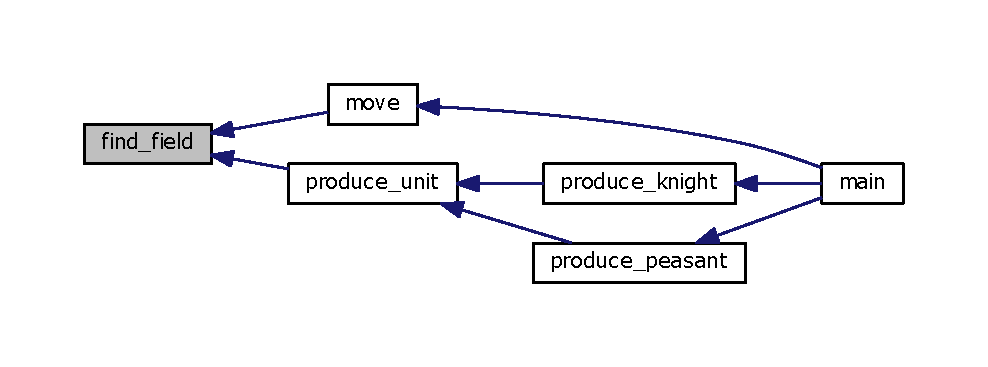
\includegraphics[width=350pt]{engine_8h_a548fff34b91e10f9ff3779c15a10ef93_icgraph}
\end{center}
\end{figure}


\hypertarget{engine_8h_a04919bedca6c747ff007c23783d37d28}{\index{engine.\-h@{engine.\-h}!incorrect\-\_\-command@{incorrect\-\_\-command}}
\index{incorrect\-\_\-command@{incorrect\-\_\-command}!engine.h@{engine.\-h}}
\subsubsection[{incorrect\-\_\-command}]{\setlength{\rightskip}{0pt plus 5cm}void incorrect\-\_\-command (
\begin{DoxyParamCaption}
{}
\end{DoxyParamCaption}
)}}\label{engine_8h_a04919bedca6c747ff007c23783d37d28}


This function enforce incorrect command with exit(42) result. 



Oto graf wywołań dla tej funkcji\-:\nopagebreak
\begin{figure}[H]
\begin{center}
\leavevmode
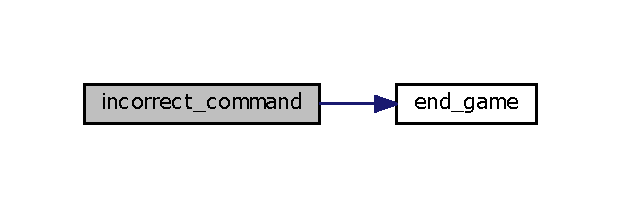
\includegraphics[width=298pt]{engine_8h_a04919bedca6c747ff007c23783d37d28_cgraph}
\end{center}
\end{figure}




Oto graf wywoływań tej funkcji\-:\nopagebreak
\begin{figure}[H]
\begin{center}
\leavevmode
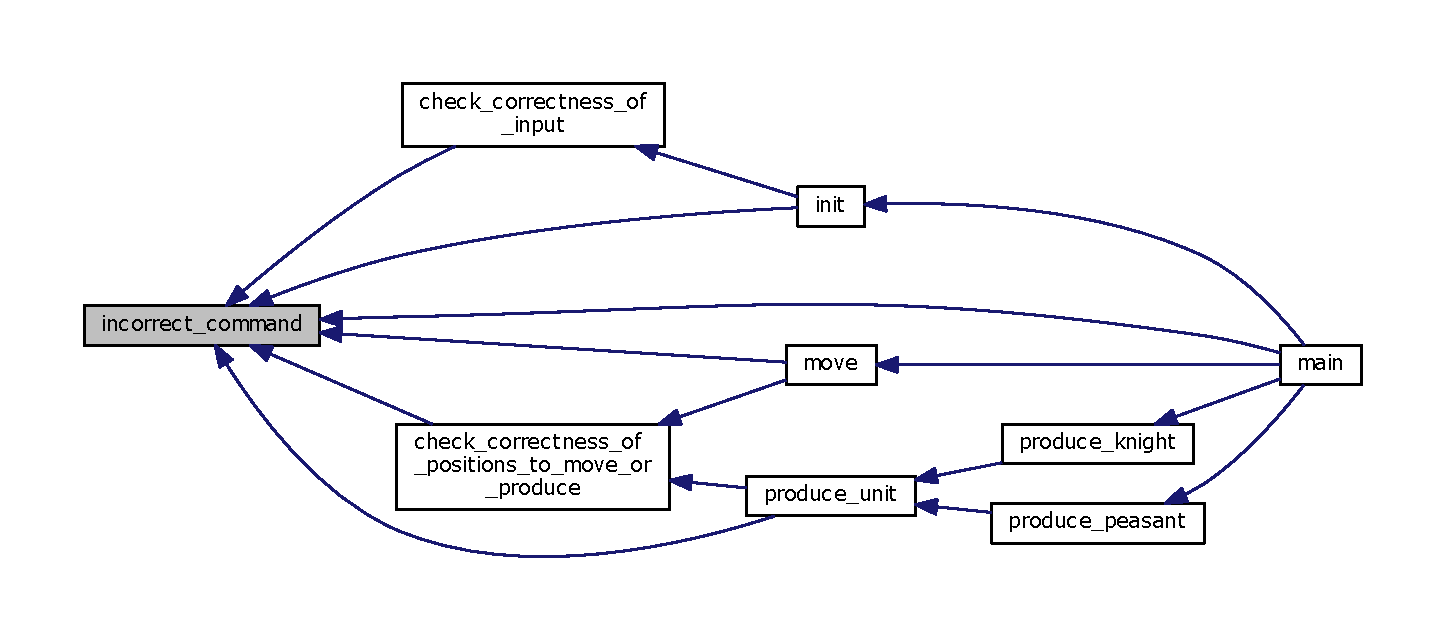
\includegraphics[width=350pt]{engine_8h_a04919bedca6c747ff007c23783d37d28_icgraph}
\end{center}
\end{figure}


\hypertarget{engine_8h_a512751eb67e971e92a205e39ee8dfe57}{\index{engine.\-h@{engine.\-h}!init@{init}}
\index{init@{init}!engine.h@{engine.\-h}}
\subsubsection[{init}]{\setlength{\rightskip}{0pt plus 5cm}void init (
\begin{DoxyParamCaption}
\item[{int}]{n, }
\item[{int}]{k, }
\item[{int}]{p, }
\item[{int}]{x1, }
\item[{int}]{y1, }
\item[{int}]{x2, }
\item[{int}]{y2}
\end{DoxyParamCaption}
)}}\label{engine_8h_a512751eb67e971e92a205e39ee8dfe57}


Initializes a game with size of a board, number of rounds and positions of kings. 



Oto graf wywołań dla tej funkcji\-:\nopagebreak
\begin{figure}[H]
\begin{center}
\leavevmode
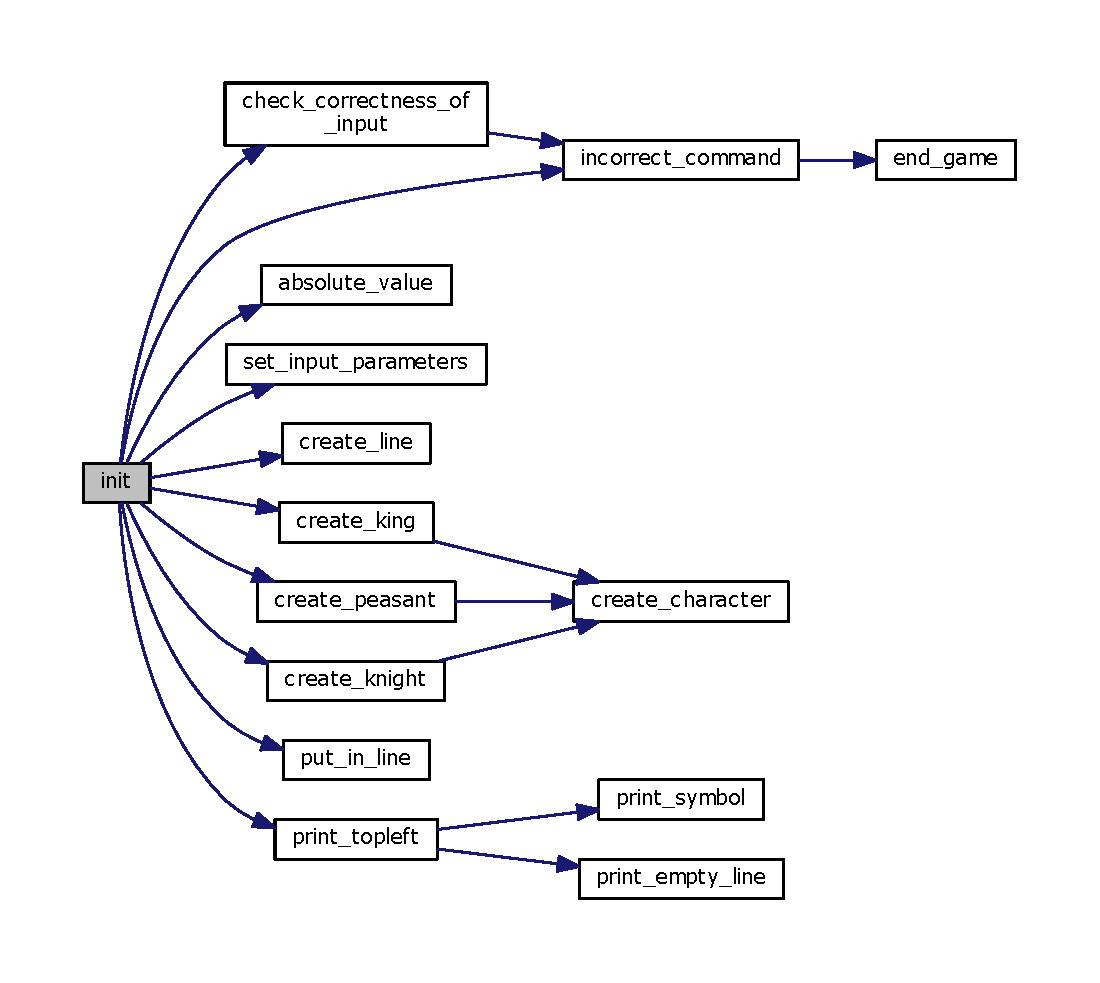
\includegraphics[width=350pt]{engine_8h_a512751eb67e971e92a205e39ee8dfe57_cgraph}
\end{center}
\end{figure}




Oto graf wywoływań tej funkcji\-:\nopagebreak
\begin{figure}[H]
\begin{center}
\leavevmode
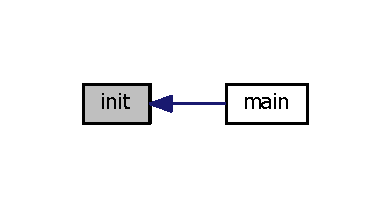
\includegraphics[width=188pt]{engine_8h_a512751eb67e971e92a205e39ee8dfe57_icgraph}
\end{center}
\end{figure}


\hypertarget{engine_8h_ab83db01d3f4a456157ab67717e594062}{\index{engine.\-h@{engine.\-h}!make\-\_\-list\-\_\-empty@{make\-\_\-list\-\_\-empty}}
\index{make\-\_\-list\-\_\-empty@{make\-\_\-list\-\_\-empty}!engine.h@{engine.\-h}}
\subsubsection[{make\-\_\-list\-\_\-empty}]{\setlength{\rightskip}{0pt plus 5cm}void make\-\_\-list\-\_\-empty (
\begin{DoxyParamCaption}
\item[{{\bf type\-\_\-of\-\_\-list\-\_\-of\-\_\-lines} $\ast$}]{constructor\-\_\-of\-\_\-main\-\_\-list}
\end{DoxyParamCaption}
)}}\label{engine_8h_ab83db01d3f4a456157ab67717e594062}


This function makes main list empty, with no previous, and next field. 


\begin{DoxyParams}[1]{Parametry}
\mbox{\tt in}  & {\em $\ast$constructor\-\_\-of\-\_\-main\-\_\-list} & Pointer to field which is mock for main\-\_\-list \\
\hline
\end{DoxyParams}


Oto graf wywoływań tej funkcji\-:\nopagebreak
\begin{figure}[H]
\begin{center}
\leavevmode
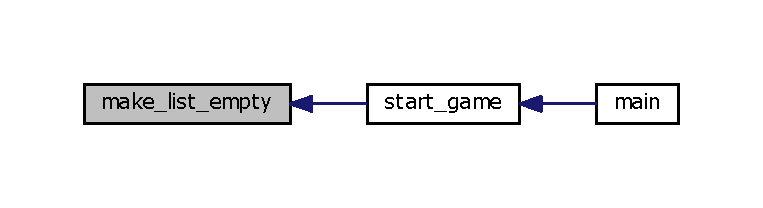
\includegraphics[width=350pt]{engine_8h_ab83db01d3f4a456157ab67717e594062_icgraph}
\end{center}
\end{figure}


\hypertarget{engine_8h_a484a4ab3480af45c873b3333f0cacee1}{\index{engine.\-h@{engine.\-h}!move@{move}}
\index{move@{move}!engine.h@{engine.\-h}}
\subsubsection[{move}]{\setlength{\rightskip}{0pt plus 5cm}void move (
\begin{DoxyParamCaption}
\item[{int}]{x1, }
\item[{int}]{y1, }
\item[{int}]{x2, }
\item[{int}]{y2}
\end{DoxyParamCaption}
)}}\label{engine_8h_a484a4ab3480af45c873b3333f0cacee1}


This function move characters from place coordinates (x1, y1) to (x2, y2) if it is possible. 

If on field with coordinates (x2, y2) is enemy unit, this function makes a fight between them. 
\begin{DoxyParams}[1]{Parametry}
\mbox{\tt in}  & {\em x1} & Column number before a move. \\
\hline
\mbox{\tt in}  & {\em y1} & Row number before a move. \\
\hline
\mbox{\tt in}  & {\em x2} & Column number after a move. \\
\hline
\mbox{\tt in}  & {\em y2} & Row number before a move. \\
\hline
\end{DoxyParams}


Oto graf wywołań dla tej funkcji\-:\nopagebreak
\begin{figure}[H]
\begin{center}
\leavevmode
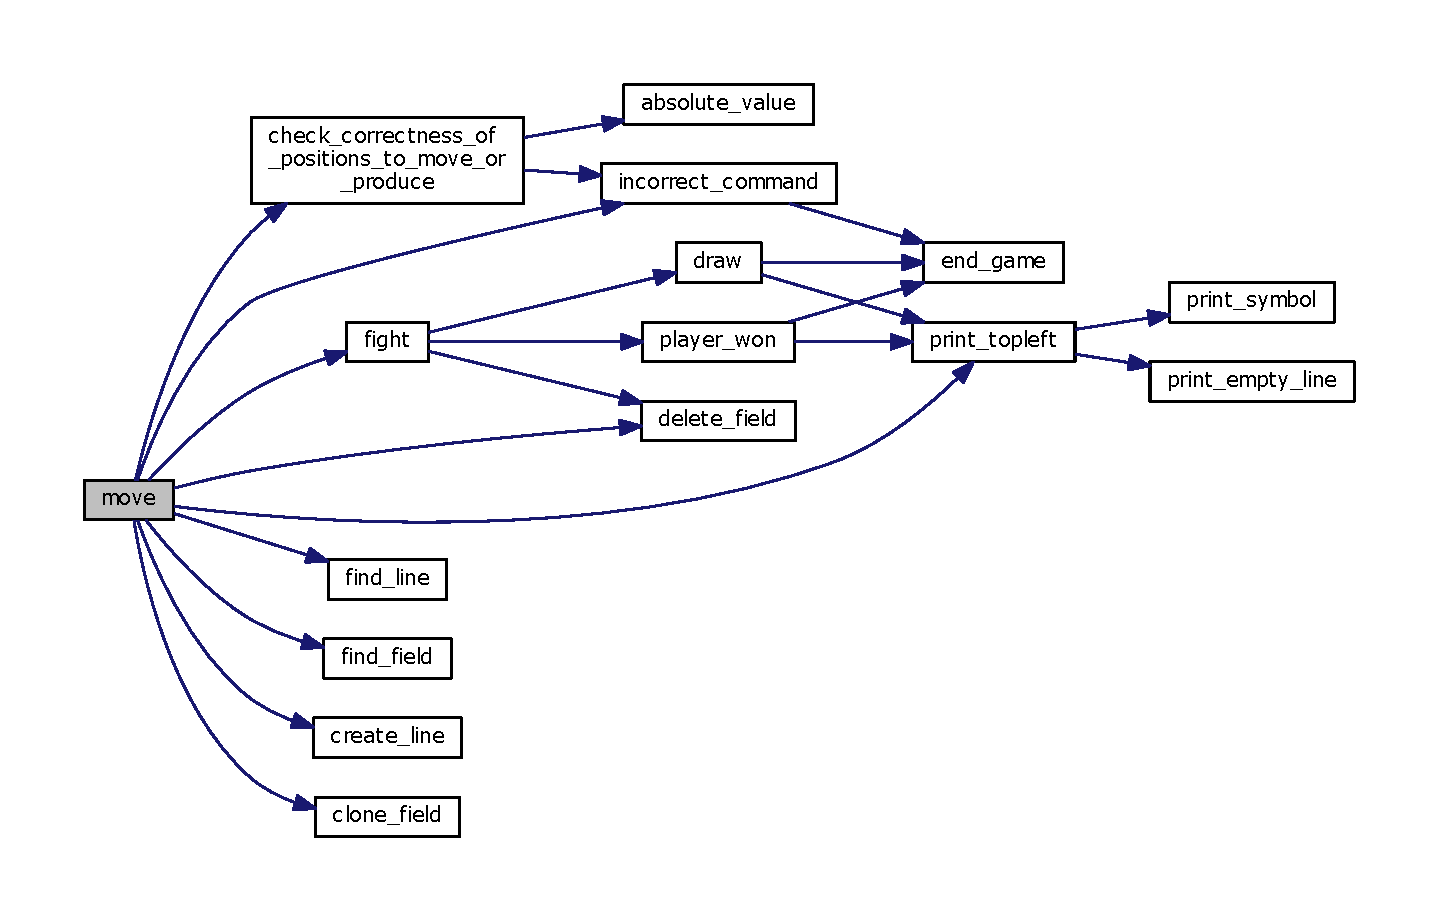
\includegraphics[width=350pt]{engine_8h_a484a4ab3480af45c873b3333f0cacee1_cgraph}
\end{center}
\end{figure}




Oto graf wywoływań tej funkcji\-:\nopagebreak
\begin{figure}[H]
\begin{center}
\leavevmode
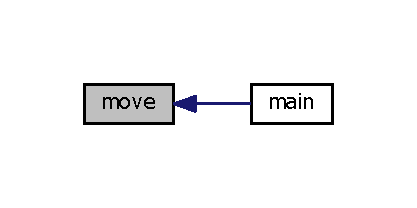
\includegraphics[width=200pt]{engine_8h_a484a4ab3480af45c873b3333f0cacee1_icgraph}
\end{center}
\end{figure}


\hypertarget{engine_8h_a32951a11c14553f0e03ed2e7576f2748}{\index{engine.\-h@{engine.\-h}!player\-\_\-won@{player\-\_\-won}}
\index{player\-\_\-won@{player\-\_\-won}!engine.h@{engine.\-h}}
\subsubsection[{player\-\_\-won}]{\setlength{\rightskip}{0pt plus 5cm}void player\-\_\-won (
\begin{DoxyParamCaption}
\item[{int}]{player\-\_\-number}
\end{DoxyParamCaption}
)}}\label{engine_8h_a32951a11c14553f0e03ed2e7576f2748}


This function end game with win result of one of players. 


\begin{DoxyParams}[1]{Parametry}
\mbox{\tt in}  & {\em player\-\_\-number} & Number of player which won. \\
\hline
\end{DoxyParams}


Oto graf wywołań dla tej funkcji\-:\nopagebreak
\begin{figure}[H]
\begin{center}
\leavevmode
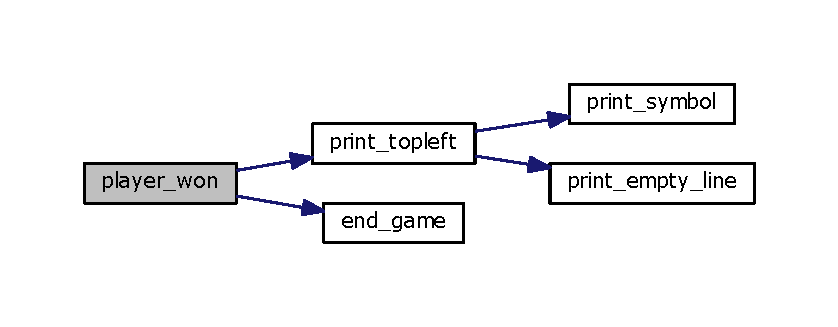
\includegraphics[width=350pt]{engine_8h_a32951a11c14553f0e03ed2e7576f2748_cgraph}
\end{center}
\end{figure}




Oto graf wywoływań tej funkcji\-:\nopagebreak
\begin{figure}[H]
\begin{center}
\leavevmode
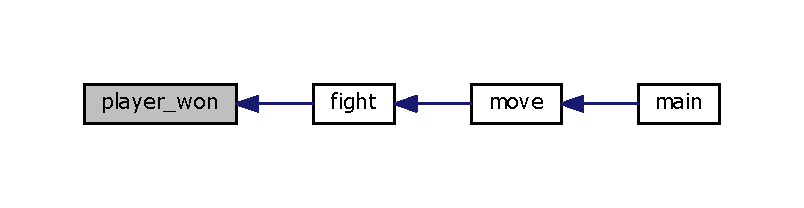
\includegraphics[width=350pt]{engine_8h_a32951a11c14553f0e03ed2e7576f2748_icgraph}
\end{center}
\end{figure}


\hypertarget{engine_8h_a6351fcf47fb1cd042b83da768706e567}{\index{engine.\-h@{engine.\-h}!print\-\_\-empty\-\_\-line@{print\-\_\-empty\-\_\-line}}
\index{print\-\_\-empty\-\_\-line@{print\-\_\-empty\-\_\-line}!engine.h@{engine.\-h}}
\subsubsection[{print\-\_\-empty\-\_\-line}]{\setlength{\rightskip}{0pt plus 5cm}void print\-\_\-empty\-\_\-line (
\begin{DoxyParamCaption}
\item[{int}]{size\-\_\-to\-\_\-print}
\end{DoxyParamCaption}
)}}\label{engine_8h_a6351fcf47fb1cd042b83da768706e567}


This function print empty line (line full of spaces) which include given amount of spaces. 


\begin{DoxyParams}[1]{Parametry}
\mbox{\tt in}  & {\em size\-\_\-to\-\_\-print} & Amount of spaces to print. \\
\hline
\end{DoxyParams}


Oto graf wywoływań tej funkcji\-:\nopagebreak
\begin{figure}[H]
\begin{center}
\leavevmode
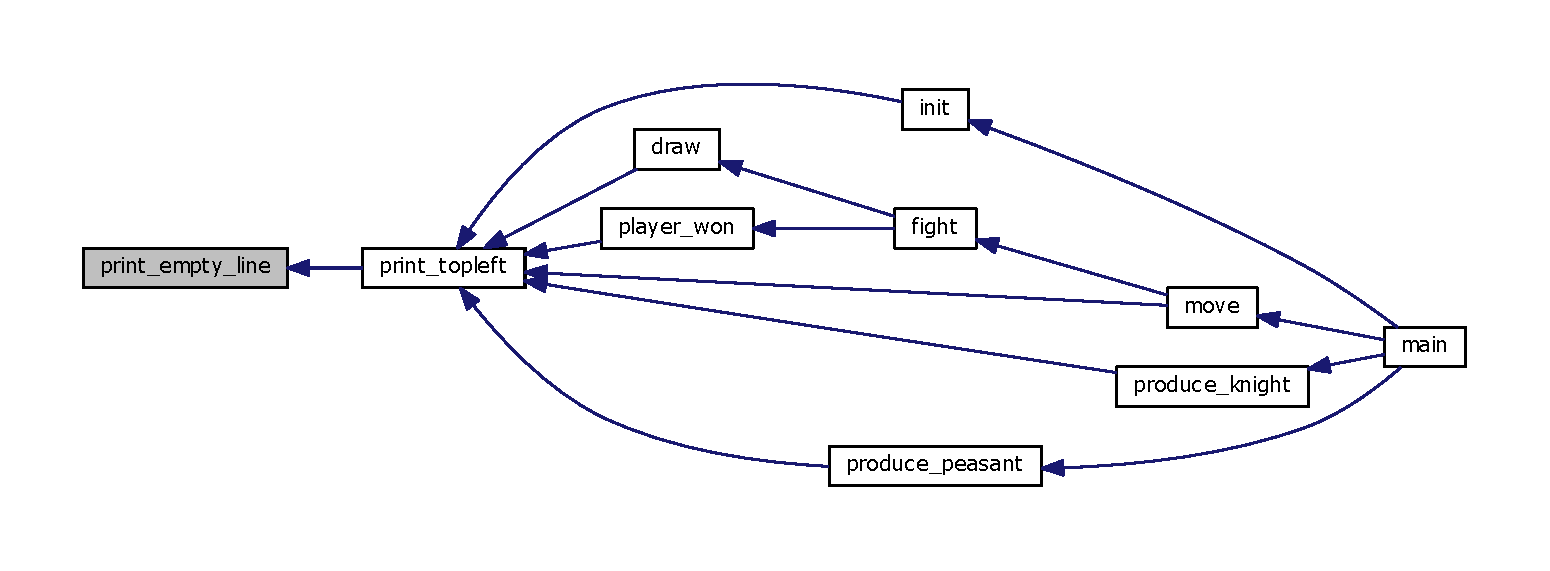
\includegraphics[width=350pt]{engine_8h_a6351fcf47fb1cd042b83da768706e567_icgraph}
\end{center}
\end{figure}


\hypertarget{engine_8h_a61500581d49ed801deeaa1b0e1c4710d}{\index{engine.\-h@{engine.\-h}!print\-\_\-symbol@{print\-\_\-symbol}}
\index{print\-\_\-symbol@{print\-\_\-symbol}!engine.h@{engine.\-h}}
\subsubsection[{print\-\_\-symbol}]{\setlength{\rightskip}{0pt plus 5cm}void print\-\_\-symbol (
\begin{DoxyParamCaption}
\item[{{\bf type\-\_\-of\-\_\-line} $\ast$}]{iterator\-\_\-on\-\_\-line}
\end{DoxyParamCaption}
)}}\label{engine_8h_a61500581d49ed801deeaa1b0e1c4710d}


This function print symbol of given field. 


\begin{DoxyParams}[1]{Parametry}
\mbox{\tt in}  & {\em $\ast$iterator\-\_\-on\-\_\-line} & Given field. \\
\hline
\end{DoxyParams}


Oto graf wywoływań tej funkcji\-:\nopagebreak
\begin{figure}[H]
\begin{center}
\leavevmode
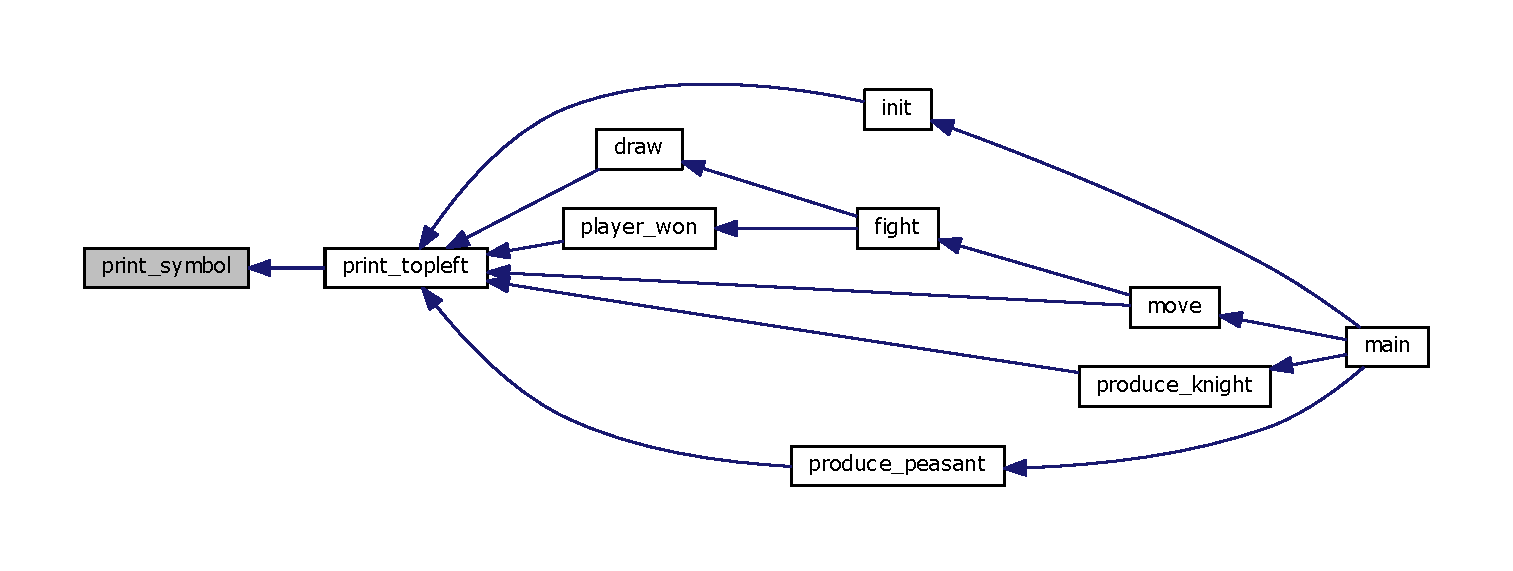
\includegraphics[width=350pt]{engine_8h_a61500581d49ed801deeaa1b0e1c4710d_icgraph}
\end{center}
\end{figure}


\hypertarget{engine_8h_a1fb95c1cfdb44f81d4ba80658b50913d}{\index{engine.\-h@{engine.\-h}!print\-\_\-topleft@{print\-\_\-topleft}}
\index{print\-\_\-topleft@{print\-\_\-topleft}!engine.h@{engine.\-h}}
\subsubsection[{print\-\_\-topleft}]{\setlength{\rightskip}{0pt plus 5cm}void print\-\_\-topleft (
\begin{DoxyParamCaption}
{}
\end{DoxyParamCaption}
)}}\label{engine_8h_a1fb95c1cfdb44f81d4ba80658b50913d}


Prints (into stdout) top-\/left corner of the board of size m x m where m = min(n,10). 



Oto graf wywołań dla tej funkcji\-:\nopagebreak
\begin{figure}[H]
\begin{center}
\leavevmode
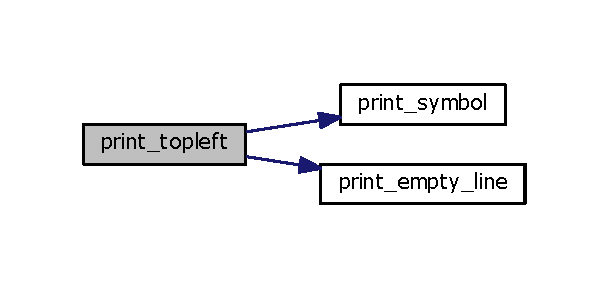
\includegraphics[width=292pt]{engine_8h_a1fb95c1cfdb44f81d4ba80658b50913d_cgraph}
\end{center}
\end{figure}




Oto graf wywoływań tej funkcji\-:\nopagebreak
\begin{figure}[H]
\begin{center}
\leavevmode
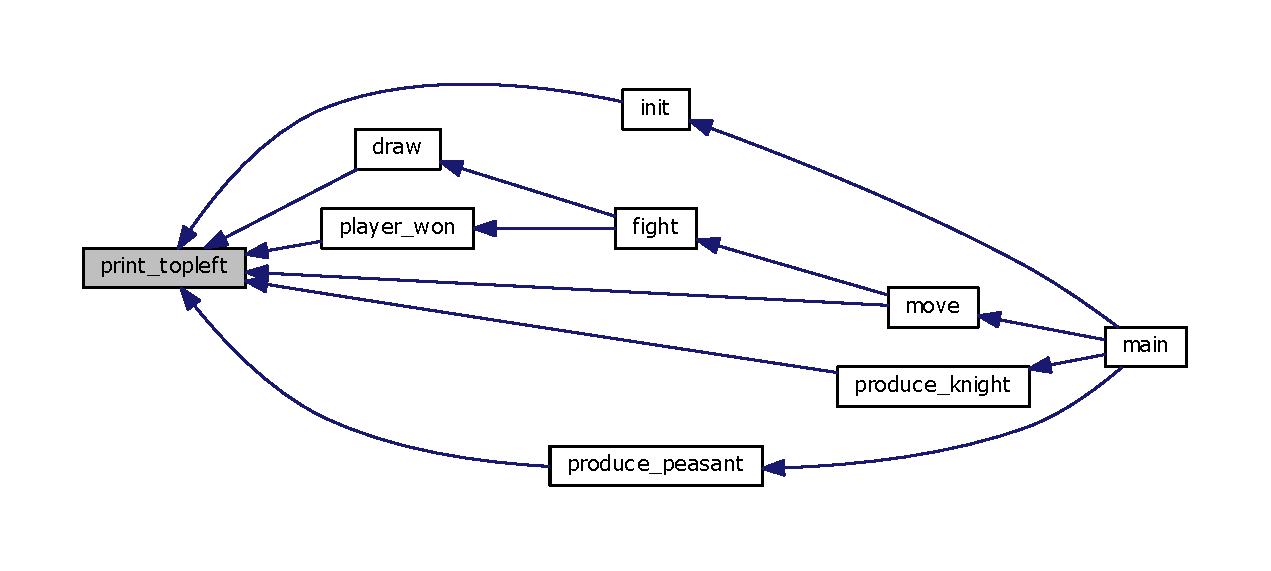
\includegraphics[width=350pt]{engine_8h_a1fb95c1cfdb44f81d4ba80658b50913d_icgraph}
\end{center}
\end{figure}


\hypertarget{engine_8h_ab6b332d9aad7c1d874fa9ca3c8e13d05}{\index{engine.\-h@{engine.\-h}!produce\-\_\-knight@{produce\-\_\-knight}}
\index{produce\-\_\-knight@{produce\-\_\-knight}!engine.h@{engine.\-h}}
\subsubsection[{produce\-\_\-knight}]{\setlength{\rightskip}{0pt plus 5cm}void produce\-\_\-knight (
\begin{DoxyParamCaption}
\item[{int}]{x1, }
\item[{int}]{y1, }
\item[{int}]{x2, }
\item[{int}]{y2}
\end{DoxyParamCaption}
)}}\label{engine_8h_ab6b332d9aad7c1d874fa9ca3c8e13d05}


This function produce unit using produce\-\_\-unit(x1, y1, x2, y2) function and give to this unit knight attribute. 


\begin{DoxyParams}[1]{Parametry}
\mbox{\tt in}  & {\em x1} & Column number of peasant which produce knight. \\
\hline
\mbox{\tt in}  & {\em y1} & Row number of peasant which produce knight. \\
\hline
\mbox{\tt in}  & {\em x2} & Column number of place to produce knight. \\
\hline
\mbox{\tt in}  & {\em y2} & Row number of place to produce knight. \\
\hline
\end{DoxyParams}


Oto graf wywołań dla tej funkcji\-:\nopagebreak
\begin{figure}[H]
\begin{center}
\leavevmode
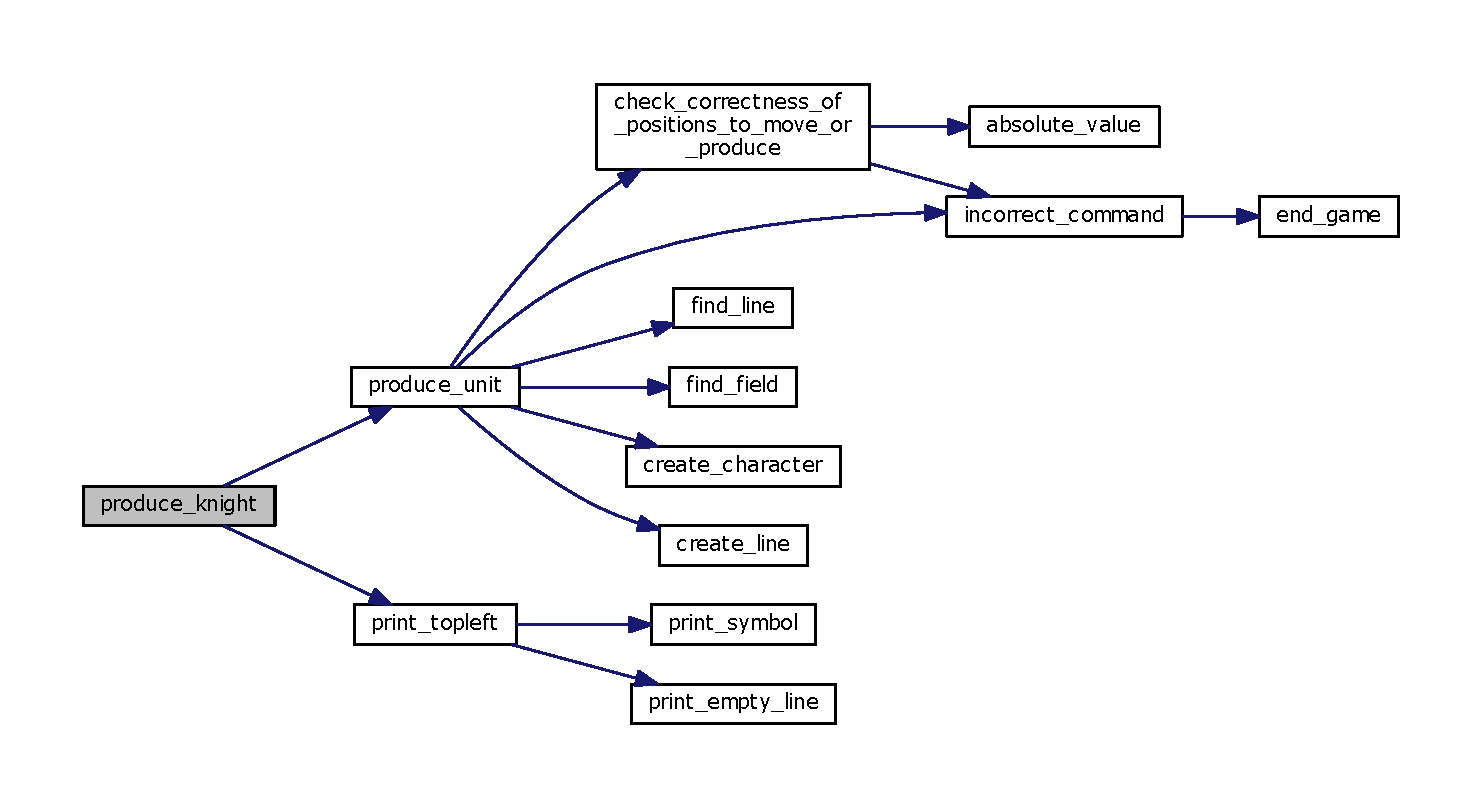
\includegraphics[width=350pt]{engine_8h_ab6b332d9aad7c1d874fa9ca3c8e13d05_cgraph}
\end{center}
\end{figure}




Oto graf wywoływań tej funkcji\-:\nopagebreak
\begin{figure}[H]
\begin{center}
\leavevmode
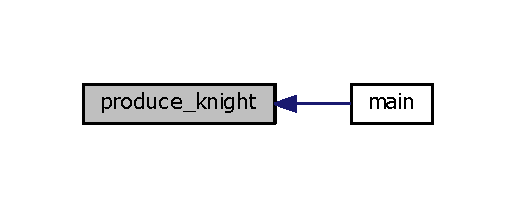
\includegraphics[width=248pt]{engine_8h_ab6b332d9aad7c1d874fa9ca3c8e13d05_icgraph}
\end{center}
\end{figure}


\hypertarget{engine_8h_abb4d3708d6bdc644d179a3630518a2b2}{\index{engine.\-h@{engine.\-h}!produce\-\_\-peasant@{produce\-\_\-peasant}}
\index{produce\-\_\-peasant@{produce\-\_\-peasant}!engine.h@{engine.\-h}}
\subsubsection[{produce\-\_\-peasant}]{\setlength{\rightskip}{0pt plus 5cm}void produce\-\_\-peasant (
\begin{DoxyParamCaption}
\item[{int}]{x1, }
\item[{int}]{y1, }
\item[{int}]{x2, }
\item[{int}]{y2}
\end{DoxyParamCaption}
)}}\label{engine_8h_abb4d3708d6bdc644d179a3630518a2b2}


This function produce unit using produce\-\_\-unit(x1, y1, x2, y2) function and give to this unit peasant attribute. 


\begin{DoxyParams}[1]{Parametry}
\mbox{\tt in}  & {\em x1} & Column number of peasant which produce peasant. \\
\hline
\mbox{\tt in}  & {\em y1} & Row number of peasant which produce peasant. \\
\hline
\mbox{\tt in}  & {\em x2} & Column number of place to produce peasant. \\
\hline
\mbox{\tt in}  & {\em y2} & Row number of place to produce peasant. \\
\hline
\end{DoxyParams}


Oto graf wywołań dla tej funkcji\-:\nopagebreak
\begin{figure}[H]
\begin{center}
\leavevmode
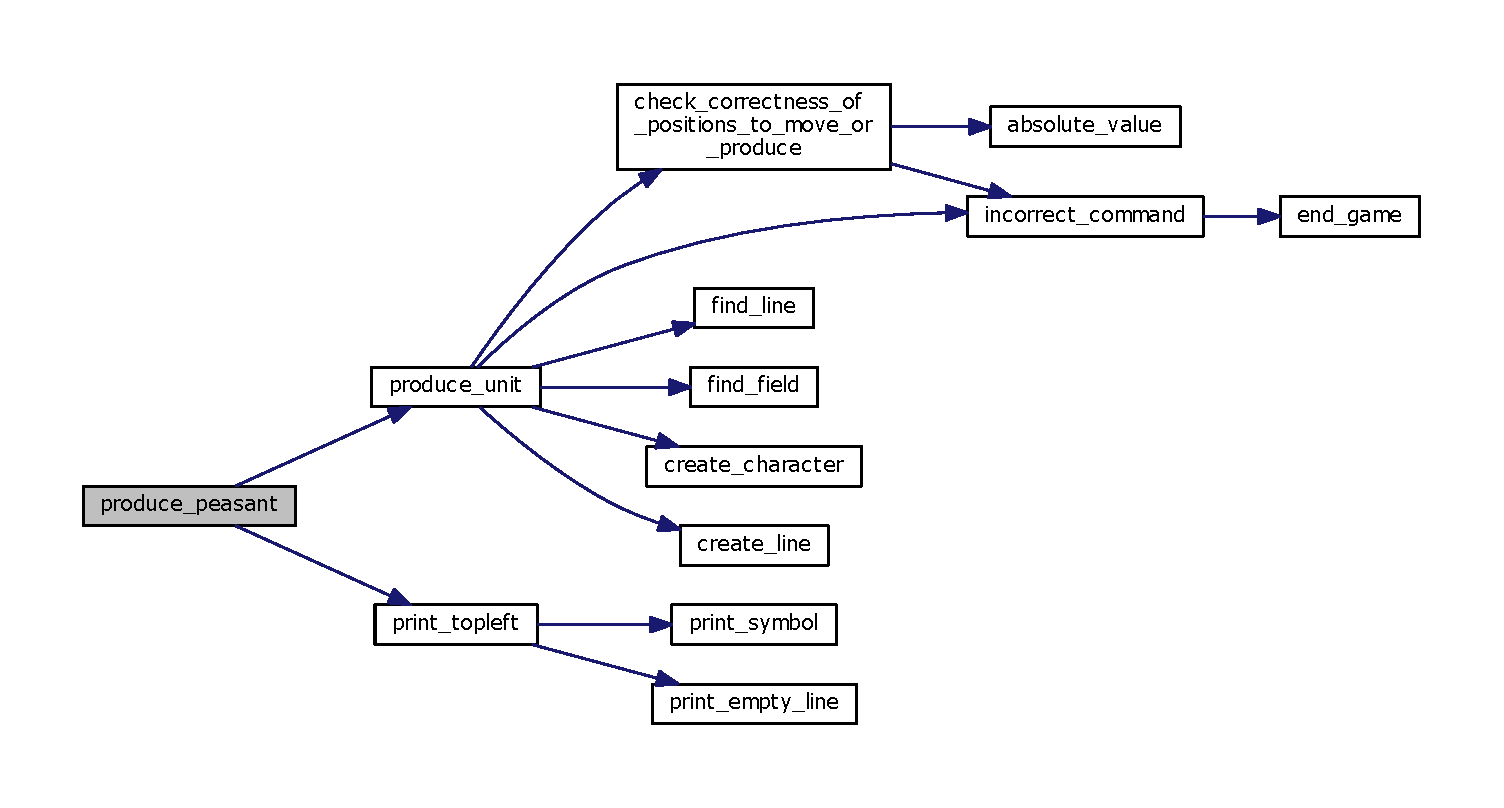
\includegraphics[width=350pt]{engine_8h_abb4d3708d6bdc644d179a3630518a2b2_cgraph}
\end{center}
\end{figure}




Oto graf wywoływań tej funkcji\-:\nopagebreak
\begin{figure}[H]
\begin{center}
\leavevmode
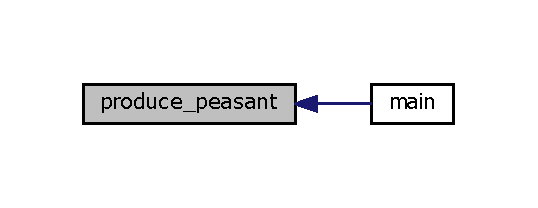
\includegraphics[width=258pt]{engine_8h_abb4d3708d6bdc644d179a3630518a2b2_icgraph}
\end{center}
\end{figure}


\hypertarget{engine_8h_a33a2165cf3d1a1dbfed5422b2226a0d7}{\index{engine.\-h@{engine.\-h}!produce\-\_\-unit@{produce\-\_\-unit}}
\index{produce\-\_\-unit@{produce\-\_\-unit}!engine.h@{engine.\-h}}
\subsubsection[{produce\-\_\-unit}]{\setlength{\rightskip}{0pt plus 5cm}{\bf type\-\_\-of\-\_\-line}$\ast$ produce\-\_\-unit (
\begin{DoxyParamCaption}
\item[{int}]{x1, }
\item[{int}]{y1, }
\item[{int}]{x2, }
\item[{int}]{y2}
\end{DoxyParamCaption}
)}}\label{engine_8h_a33a2165cf3d1a1dbfed5422b2226a0d7}


This function results in production unit on field with coordinates (x2, y2) by peasant on field with coordinates (x1, y1) 


\begin{DoxyParams}[1]{Parametry}
\mbox{\tt in}  & {\em x1} & Column number of peasant which produce unit. \\
\hline
\mbox{\tt in}  & {\em y1} & Row number of peasant which produce unit. \\
\hline
\mbox{\tt in}  & {\em x2} & Column number of place to produce unit. \\
\hline
\mbox{\tt in}  & {\em y2} & Row number of place to produce unit. \\
\hline
\end{DoxyParams}


Oto graf wywołań dla tej funkcji\-:\nopagebreak
\begin{figure}[H]
\begin{center}
\leavevmode
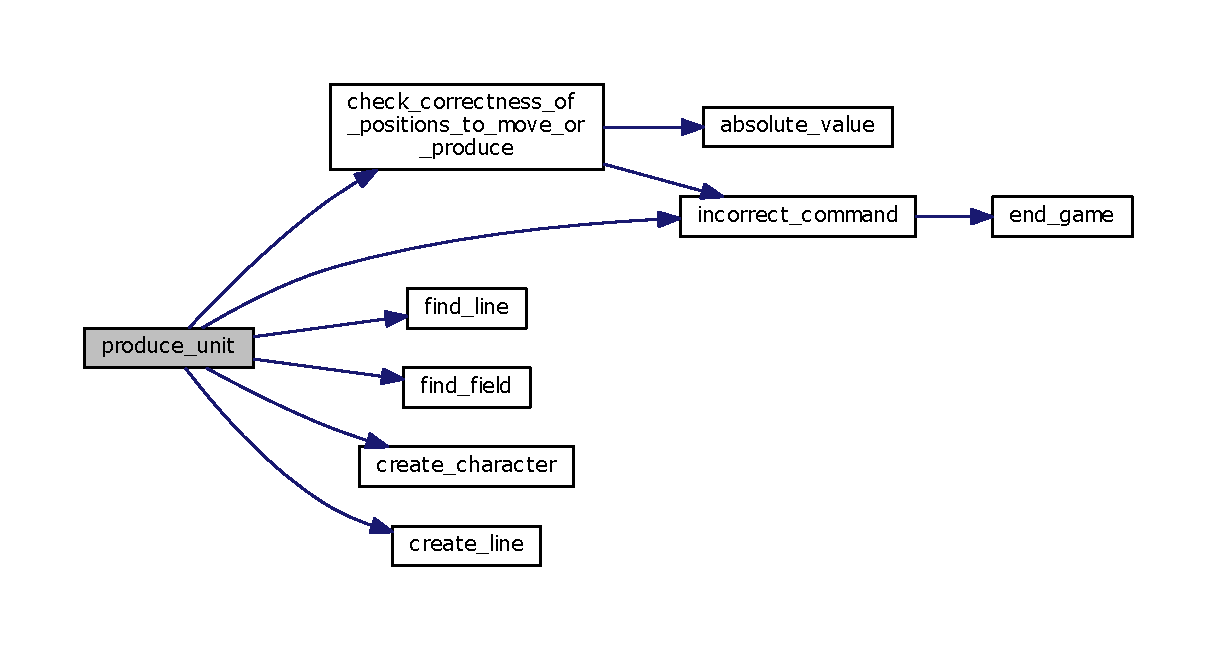
\includegraphics[width=350pt]{engine_8h_a33a2165cf3d1a1dbfed5422b2226a0d7_cgraph}
\end{center}
\end{figure}




Oto graf wywoływań tej funkcji\-:\nopagebreak
\begin{figure}[H]
\begin{center}
\leavevmode
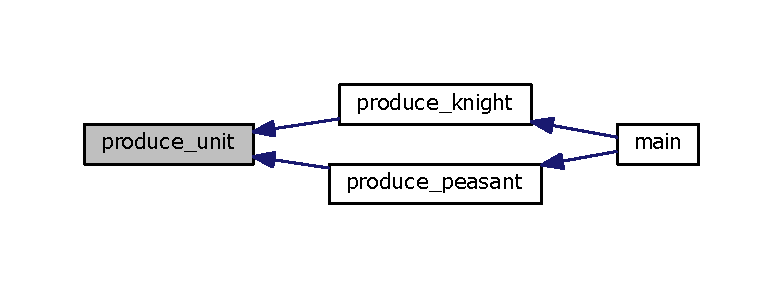
\includegraphics[width=350pt]{engine_8h_a33a2165cf3d1a1dbfed5422b2226a0d7_icgraph}
\end{center}
\end{figure}


\hypertarget{engine_8h_a356d8f07535e1016fbe5a6fdddb33516}{\index{engine.\-h@{engine.\-h}!put\-\_\-in\-\_\-line@{put\-\_\-in\-\_\-line}}
\index{put\-\_\-in\-\_\-line@{put\-\_\-in\-\_\-line}!engine.h@{engine.\-h}}
\subsubsection[{put\-\_\-in\-\_\-line}]{\setlength{\rightskip}{0pt plus 5cm}void put\-\_\-in\-\_\-line (
\begin{DoxyParamCaption}
\item[{{\bf type\-\_\-of\-\_\-line} $\ast$}]{new\-\_\-line1, }
\item[{{\bf type\-\_\-of\-\_\-line} $\ast$}]{king, }
\item[{{\bf type\-\_\-of\-\_\-line} $\ast$}]{peasant, }
\item[{{\bf type\-\_\-of\-\_\-line} $\ast$}]{knight1, }
\item[{{\bf type\-\_\-of\-\_\-line} $\ast$}]{knight2}
\end{DoxyParamCaption}
)}}\label{engine_8h_a356d8f07535e1016fbe5a6fdddb33516}


This function put king, peasant, knight1 and knigth2 to line behind new\-\_\-line1. 



Oto graf wywoływań tej funkcji\-:\nopagebreak
\begin{figure}[H]
\begin{center}
\leavevmode
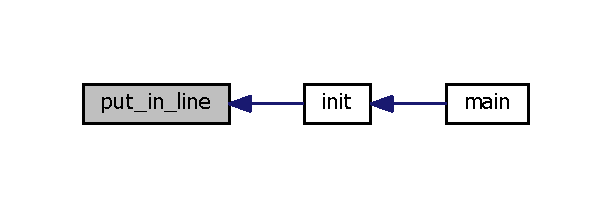
\includegraphics[width=294pt]{engine_8h_a356d8f07535e1016fbe5a6fdddb33516_icgraph}
\end{center}
\end{figure}


\hypertarget{engine_8h_a8e474b14265a2ebbcb0c7461817214bc}{\index{engine.\-h@{engine.\-h}!set\-\_\-input\-\_\-parameters@{set\-\_\-input\-\_\-parameters}}
\index{set\-\_\-input\-\_\-parameters@{set\-\_\-input\-\_\-parameters}!engine.h@{engine.\-h}}
\subsubsection[{set\-\_\-input\-\_\-parameters}]{\setlength{\rightskip}{0pt plus 5cm}void set\-\_\-input\-\_\-parameters (
\begin{DoxyParamCaption}
\item[{int}]{n, }
\item[{int}]{k, }
\item[{int}]{p, }
\item[{int}]{x1, }
\item[{int}]{y1, }
\item[{int}]{x2, }
\item[{int}]{y2}
\end{DoxyParamCaption}
)}}\label{engine_8h_a8e474b14265a2ebbcb0c7461817214bc}


This function memorize parameters given with I\-N\-I\-T. 



Oto graf wywoływań tej funkcji\-:\nopagebreak
\begin{figure}[H]
\begin{center}
\leavevmode
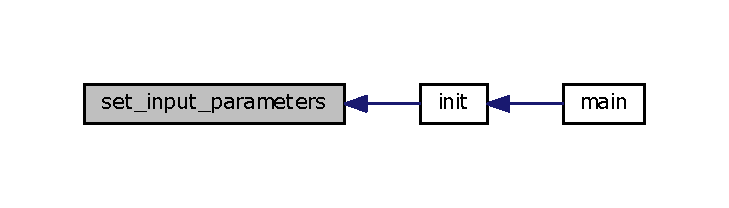
\includegraphics[width=350pt]{engine_8h_a8e474b14265a2ebbcb0c7461817214bc_icgraph}
\end{center}
\end{figure}


\hypertarget{engine_8h_a671b58f5509a3a9fa692bacccfc32cc9}{\index{engine.\-h@{engine.\-h}!start\-\_\-game@{start\-\_\-game}}
\index{start\-\_\-game@{start\-\_\-game}!engine.h@{engine.\-h}}
\subsubsection[{start\-\_\-game}]{\setlength{\rightskip}{0pt plus 5cm}void start\-\_\-game (
\begin{DoxyParamCaption}
{}
\end{DoxyParamCaption}
)}}\label{engine_8h_a671b58f5509a3a9fa692bacccfc32cc9}


Initializes a game. 

Needed before first I\-N\-I\-T. 

Oto graf wywołań dla tej funkcji\-:\nopagebreak
\begin{figure}[H]
\begin{center}
\leavevmode
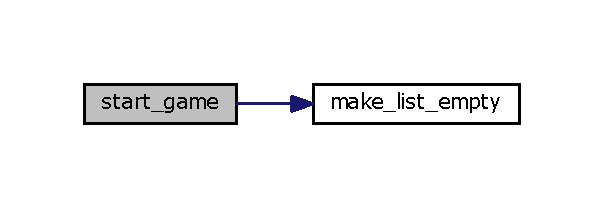
\includegraphics[width=290pt]{engine_8h_a671b58f5509a3a9fa692bacccfc32cc9_cgraph}
\end{center}
\end{figure}




Oto graf wywoływań tej funkcji\-:\nopagebreak
\begin{figure}[H]
\begin{center}
\leavevmode
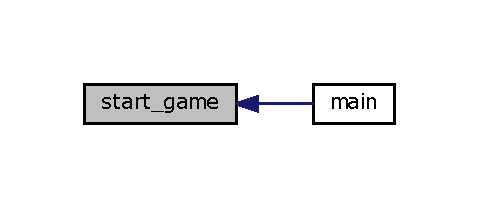
\includegraphics[width=230pt]{engine_8h_a671b58f5509a3a9fa692bacccfc32cc9_icgraph}
\end{center}
\end{figure}




\subsection{Dokumentacja zmiennych}
\hypertarget{engine_8h_a121e21e0e93b33f6071d24a43ce28830}{\index{engine.\-h@{engine.\-h}!constructor\-\_\-of\-\_\-main\-\_\-list@{constructor\-\_\-of\-\_\-main\-\_\-list}}
\index{constructor\-\_\-of\-\_\-main\-\_\-list@{constructor\-\_\-of\-\_\-main\-\_\-list}!engine.h@{engine.\-h}}
\subsubsection[{constructor\-\_\-of\-\_\-main\-\_\-list}]{\setlength{\rightskip}{0pt plus 5cm}{\bf type\-\_\-of\-\_\-list\-\_\-of\-\_\-lines}$\ast$ constructor\-\_\-of\-\_\-main\-\_\-list}}\label{engine_8h_a121e21e0e93b33f6071d24a43ce28830}


Pointer to mock of list of lines. 

\hypertarget{engine_8h_aa60bf4b5b108d9591140a5abfc89c5fb}{\index{engine.\-h@{engine.\-h}!counter\-\_\-of\-\_\-rounds@{counter\-\_\-of\-\_\-rounds}}
\index{counter\-\_\-of\-\_\-rounds@{counter\-\_\-of\-\_\-rounds}!engine.h@{engine.\-h}}
\subsubsection[{counter\-\_\-of\-\_\-rounds}]{\setlength{\rightskip}{0pt plus 5cm}int counter\-\_\-of\-\_\-rounds}}\label{engine_8h_aa60bf4b5b108d9591140a5abfc89c5fb}


Counter of actually playing turn. 

\hypertarget{engine_8h_aad242164bb0908170880af0688ed3438}{\index{engine.\-h@{engine.\-h}!input@{input}}
\index{input@{input}!engine.h@{engine.\-h}}
\subsubsection[{input}]{\setlength{\rightskip}{0pt plus 5cm}{\bf type\-\_\-of\-\_\-input\-\_\-parameters} input}}\label{engine_8h_aad242164bb0908170880af0688ed3438}


Memory of input parameters. 

\hypertarget{engine_8h_ac04a3e0434907c4977d4cc8592472e4e}{\index{engine.\-h@{engine.\-h}!number\-\_\-of\-\_\-init@{number\-\_\-of\-\_\-init}}
\index{number\-\_\-of\-\_\-init@{number\-\_\-of\-\_\-init}!engine.h@{engine.\-h}}
\subsubsection[{number\-\_\-of\-\_\-init}]{\setlength{\rightskip}{0pt plus 5cm}int number\-\_\-of\-\_\-init}}\label{engine_8h_ac04a3e0434907c4977d4cc8592472e4e}


Counter of number of initializations. 

\hypertarget{engine_8h_a230bf1ce6f1480f9fddb4577d1742f4f}{\index{engine.\-h@{engine.\-h}!player\-\_\-number@{player\-\_\-number}}
\index{player\-\_\-number@{player\-\_\-number}!engine.h@{engine.\-h}}
\subsubsection[{player\-\_\-number}]{\setlength{\rightskip}{0pt plus 5cm}int player\-\_\-number}}\label{engine_8h_a230bf1ce6f1480f9fddb4577d1742f4f}


Counter of actually playing player. 


\hypertarget{middle__ages_8c}{\section{Dokumentacja pliku middle\-\_\-ages.\-c}
\label{middle__ages_8c}\index{middle\-\_\-ages.\-c@{middle\-\_\-ages.\-c}}
}


Interface of middle\-\_\-ages.  


{\ttfamily \#include $<$stdio.\-h$>$}\\*
{\ttfamily \#include $<$string.\-h$>$}\\*
{\ttfamily \#include $<$stdlib.\-h$>$}\\*
{\ttfamily \#include $<$stdbool.\-h$>$}\\*
{\ttfamily \#include \char`\"{}parse.\-h\char`\"{}}\\*
{\ttfamily \#include \char`\"{}engine.\-h\char`\"{}}\\*
Wykres zależności załączania dla middle\-\_\-ages.\-c\-:\nopagebreak
\begin{figure}[H]
\begin{center}
\leavevmode
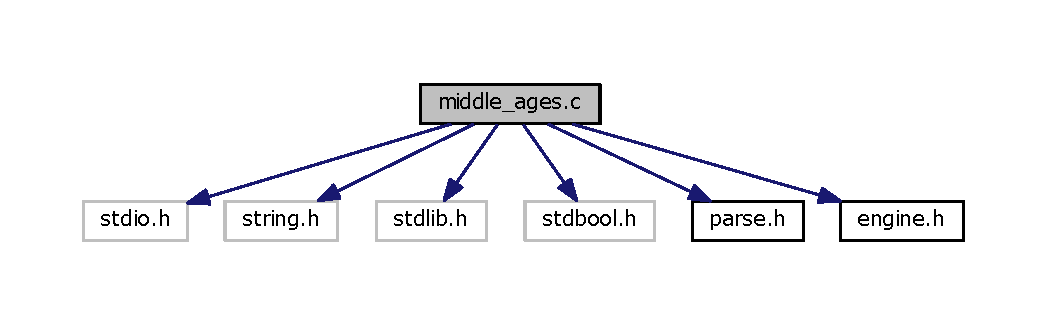
\includegraphics[width=350pt]{middle__ages_8c__incl}
\end{center}
\end{figure}
\subsection*{Funkcje}
\begin{DoxyCompactItemize}
\item 
\hypertarget{middle__ages_8c_ae66f6b31b5ad750f1fe042a706a4e3d4}{int \hyperlink{middle__ages_8c_ae66f6b31b5ad750f1fe042a706a4e3d4}{main} ()}\label{middle__ages_8c_ae66f6b31b5ad750f1fe042a706a4e3d4}

\begin{DoxyCompactList}\small\item\em Function \hyperlink{middle__ages_8c_ae66f6b31b5ad750f1fe042a706a4e3d4}{main()} gets commands, and makes them. \end{DoxyCompactList}\end{DoxyCompactItemize}


\subsection{Opis szczegółowy}
Interface of middle\-\_\-ages. 
\hypertarget{parse_8h}{\section{Dokumentacja pliku parse.\-h}
\label{parse_8h}\index{parse.\-h@{parse.\-h}}
}


Interface of parser.  


Ten wykres pokazuje, które pliki bezpośrednio lub pośrednio załączają ten plik\-:\nopagebreak
\begin{figure}[H]
\begin{center}
\leavevmode
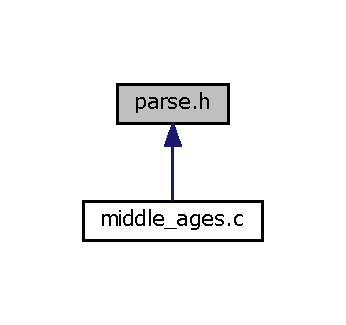
\includegraphics[width=166pt]{parse_8h__dep__incl}
\end{center}
\end{figure}
\subsection*{Struktury danych}
\begin{DoxyCompactItemize}
\item 
struct \hyperlink{structdef__command}{def\-\_\-command}
\end{DoxyCompactItemize}
\subsection*{Definicje typów}
\begin{DoxyCompactItemize}
\item 
\hypertarget{parse_8h_af0cd7b52142d459e0b082cc95c9ad293}{typedef struct \hyperlink{structdef__command}{def\-\_\-command} {\bfseries command}}\label{parse_8h_af0cd7b52142d459e0b082cc95c9ad293}

\end{DoxyCompactItemize}
\subsection*{Funkcje}
\begin{DoxyCompactItemize}
\item 
\hypertarget{parse_8h_aac0ba770012451223eb424b457dade42}{void \hyperlink{parse_8h_aac0ba770012451223eb424b457dade42}{make\-\_\-command\-\_\-incorrect} (\hyperlink{structdef__command}{command} table)}\label{parse_8h_aac0ba770012451223eb424b457dade42}

\begin{DoxyCompactList}\small\item\em This function return command with parameters correct = false. \end{DoxyCompactList}\item 
bool \hyperlink{parse_8h_a0d148e8e7eecbfdb39c375e9649c680d}{correctness\-\_\-of\-\_\-spaces} (char \hyperlink{engine_8h_aad242164bb0908170880af0688ed3438}{input}\mbox{[}102\mbox{]}, \hyperlink{structdef__command}{command} table)
\begin{DoxyCompactList}\small\item\em This function check if input has has correct spaces. \end{DoxyCompactList}\item 
\hyperlink{structdef__command}{command} \hyperlink{parse_8h_a2f338d0e0bbdffa56a0af068d184acea}{parse\-\_\-command} ()
\begin{DoxyCompactList}\small\item\em Reads a command. \end{DoxyCompactList}\end{DoxyCompactItemize}


\subsection{Opis szczegółowy}
Interface of parser. 

\subsection{Dokumentacja funkcji}
\hypertarget{parse_8h_a0d148e8e7eecbfdb39c375e9649c680d}{\index{parse.\-h@{parse.\-h}!correctness\-\_\-of\-\_\-spaces@{correctness\-\_\-of\-\_\-spaces}}
\index{correctness\-\_\-of\-\_\-spaces@{correctness\-\_\-of\-\_\-spaces}!parse.h@{parse.\-h}}
\subsubsection[{correctness\-\_\-of\-\_\-spaces}]{\setlength{\rightskip}{0pt plus 5cm}bool correctness\-\_\-of\-\_\-spaces (
\begin{DoxyParamCaption}
\item[{char}]{input\mbox{[}102\mbox{]}, }
\item[{{\bf command}}]{table}
\end{DoxyParamCaption}
)}}\label{parse_8h_a0d148e8e7eecbfdb39c375e9649c680d}


This function check if input has has correct spaces. 

Return true if it's true, and false otherwise. 

Oto graf wywoływań tej funkcji\-:\nopagebreak
\begin{figure}[H]
\begin{center}
\leavevmode
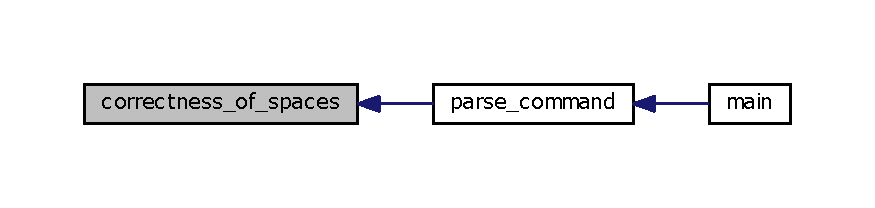
\includegraphics[width=350pt]{parse_8h_a0d148e8e7eecbfdb39c375e9649c680d_icgraph}
\end{center}
\end{figure}


\hypertarget{parse_8h_a2f338d0e0bbdffa56a0af068d184acea}{\index{parse.\-h@{parse.\-h}!parse\-\_\-command@{parse\-\_\-command}}
\index{parse\-\_\-command@{parse\-\_\-command}!parse.h@{parse.\-h}}
\subsubsection[{parse\-\_\-command}]{\setlength{\rightskip}{0pt plus 5cm}{\bf command} parse\-\_\-command (
\begin{DoxyParamCaption}
{}
\end{DoxyParamCaption}
)}}\label{parse_8h_a2f338d0e0bbdffa56a0af068d184acea}


Reads a command. 

Returns command with data points using 'command' structure. 

Oto graf wywołań dla tej funkcji\-:\nopagebreak
\begin{figure}[H]
\begin{center}
\leavevmode
\includegraphics[width=350pt]{parse_8h_a2f338d0e0bbdffa56a0af068d184acea_cgraph}
\end{center}
\end{figure}




Oto graf wywoływań tej funkcji\-:\nopagebreak
\begin{figure}[H]
\begin{center}
\leavevmode
\includegraphics[width=252pt]{parse_8h_a2f338d0e0bbdffa56a0af068d184acea_icgraph}
\end{center}
\end{figure}



%--- End generated contents ---

% Index
\newpage
\phantomsection
\addcontentsline{toc}{chapter}{Indeks}
\printindex

\end{document}
